\subsection{FOUR-SHIP}

\begin{figure}[htbp]
    \centering
    \begin{minipage}[b]{0.5\textwidth}
        \centering
        \begin{tikzpicture}[figstyle]
            
            \coordinate (1) at (0,0);
            \coordinate (2) at ($(1)+(20,0)$);
            \coordinate (3) at ($(1)+(0,-30)$);
            \coordinate (4) at ($(3)+(20,0)$);

            \draw[thin, <->]
            ($(1)+(-5,0)$) 
            -- ($(3)+(-5,0)$)
            node[font=\footnotesize, pos=0.5, rotate=90, above] {1.5-3.0 nm};
            \draw[thin]
            (1) -- ($(1)+(-7,0)$)
            (3) -- ($(3)+(-7,0)$);

            \draw[thin, <->]
            ($(1)+(0,5)$) 
            -- ($(2)+(0,5)$)
            node[font=\footnotesize, pos=0.5, above] {line abreast};
            \draw[thin]
            (1) -- ($(1)+(0,7)$)
            (2) -- ($(2)+(0,7)$);

            \draw[thin, <->]
            ($(3)+(0,5)$) 
            -- ($(4)+(0,5)$)
            node[font=\footnotesize, pos=0.5, above] {line abreast};
            \draw[thin]
            (3) -- ($(3)+(0,7)$)
            (4) -- ($(4)+(0,7)$);


            \node[yshift=-2mm] (1fig) at (1) {
                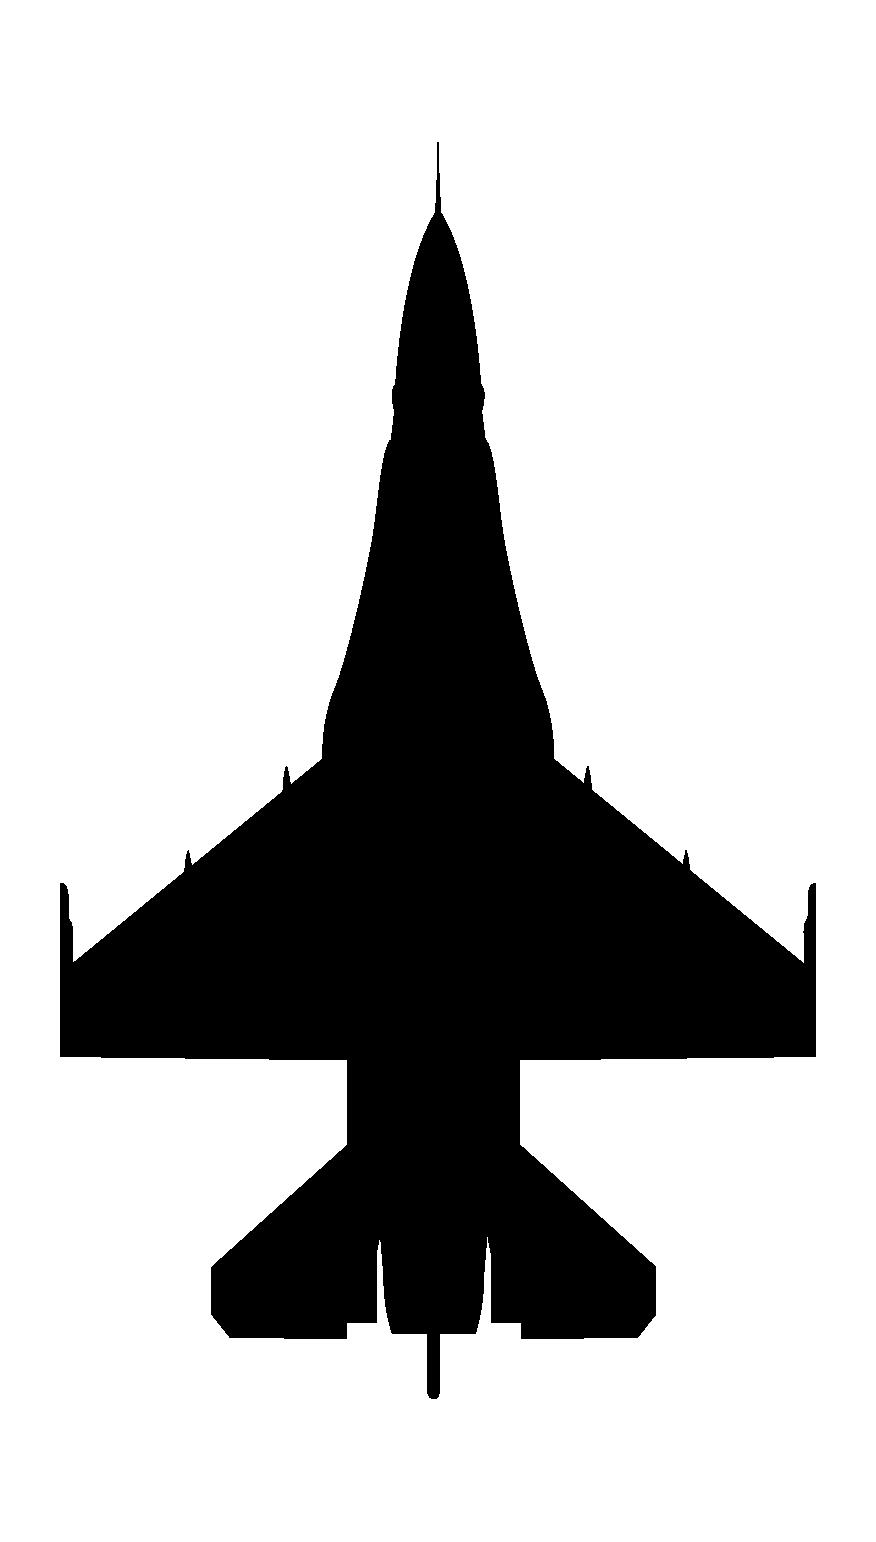
\includegraphics[
                    width=7.5mm,
                ]{diagrams/aircraft/silhouette_f16_top.pdf}
            };
            
            \node[yshift=-2mm] (2fig) at (2) {
                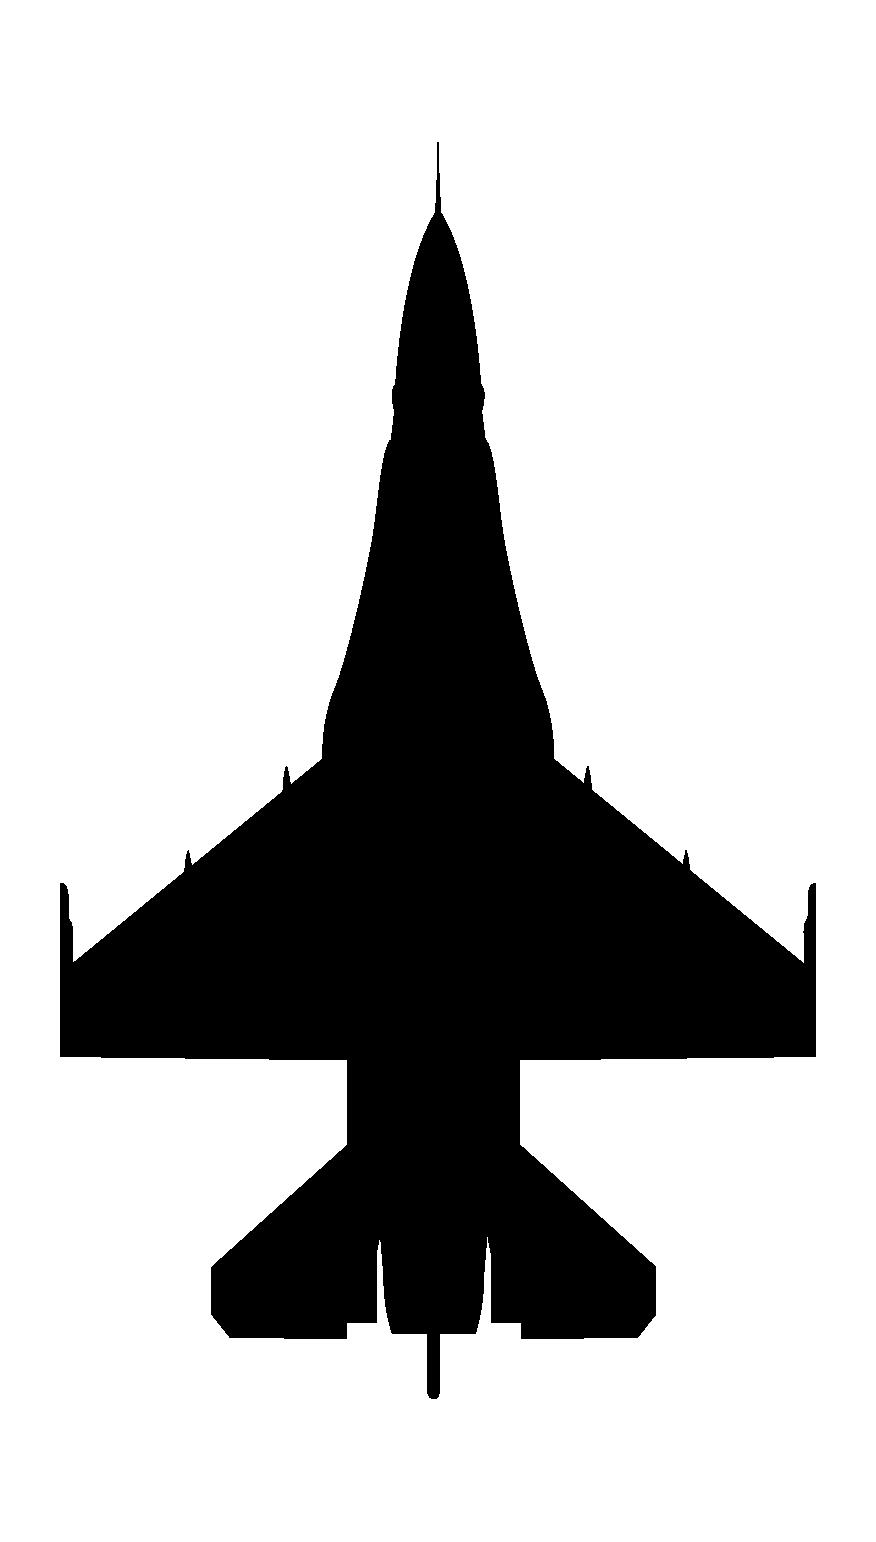
\includegraphics[
                    width=7.5mm,
                ]{diagrams/aircraft/silhouette_f16_top.pdf}
            };

            \node[yshift=-2mm] (3fig) at (3) {
                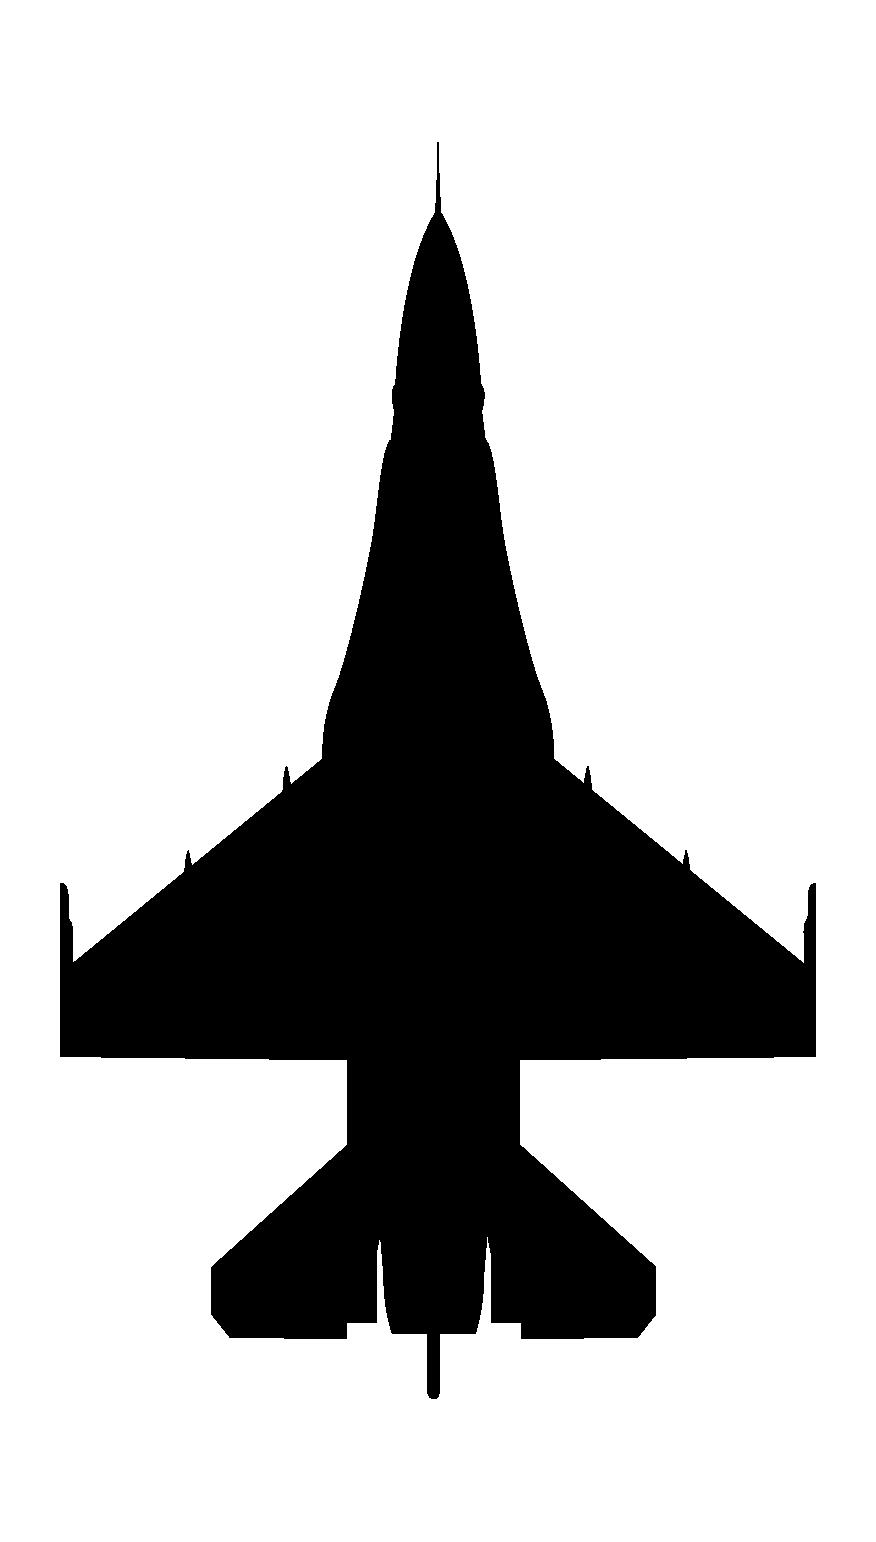
\includegraphics[
                    width=7.5mm,
                ]{diagrams/aircraft/silhouette_f16_top.pdf}
            };
            
            \node[yshift=-2mm] (4fig) at (4) {
                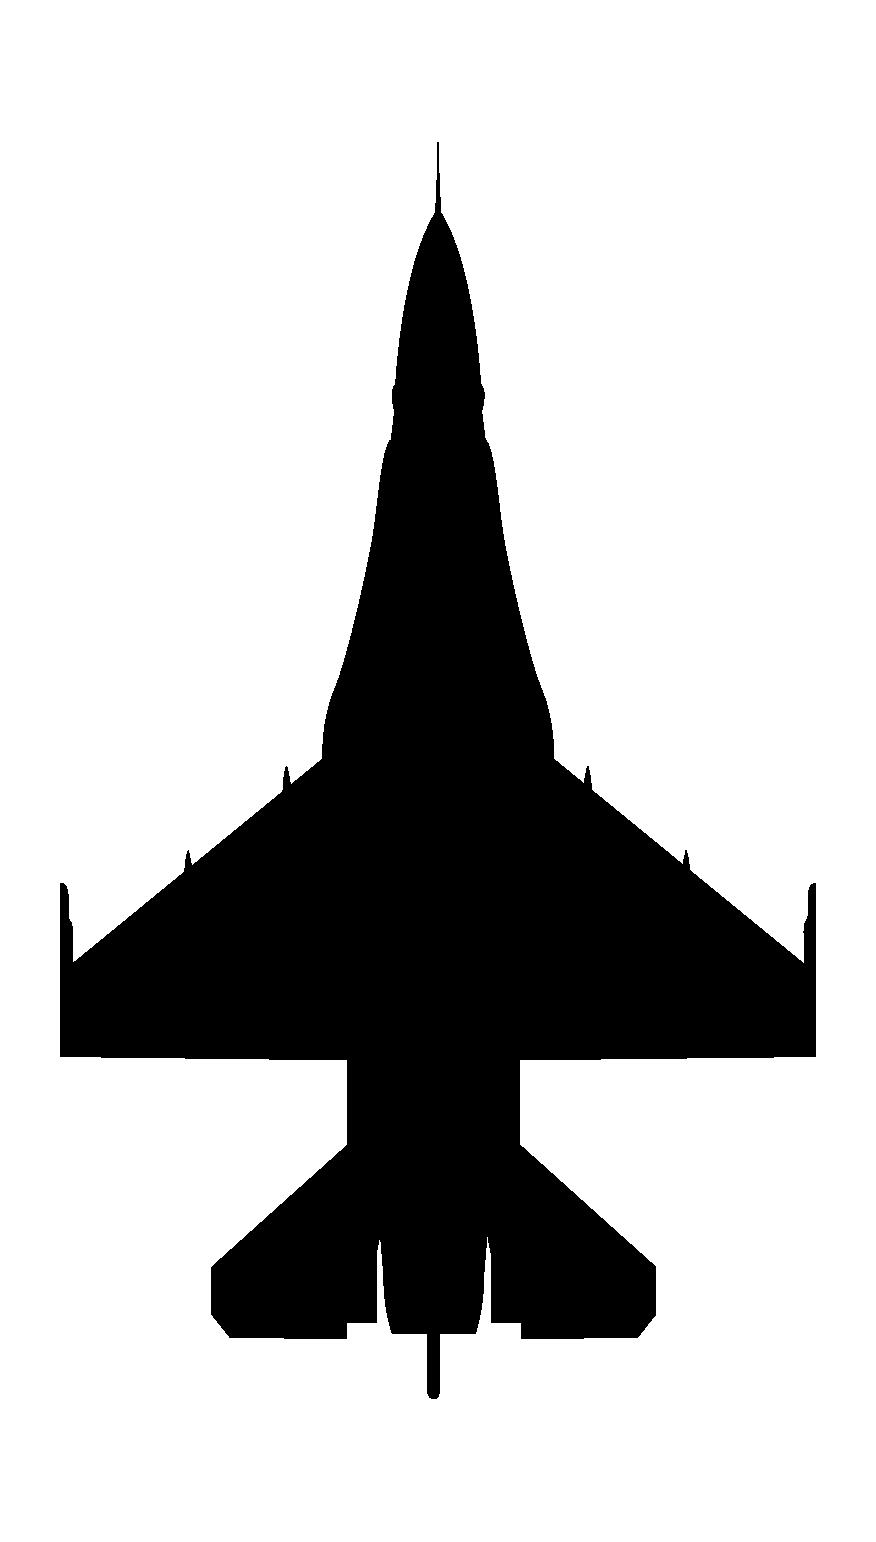
\includegraphics[
                    width=7.5mm,
                ]{diagrams/aircraft/silhouette_f16_top.pdf}
            };

            \node[anchor=north, font=\footnotesize] (1label) at (1fig.south) {1};
            \node[anchor=north, font=\footnotesize] (2label) at (2fig.south) {2};
            \node[anchor=north, font=\footnotesize] (3label) at (3fig.south) {3};
            \node[anchor=north, font=\footnotesize] (4label) at (4fig.south) {4};

        \end{tikzpicture}
        \caption{Four-ship box formation}
        \label{fig:supp_fig:form:box}
    \end{minipage}%
    \begin{minipage}[b]{0.5\textwidth}
        \centering
        \begin{tikzpicture}[figstyle]
            
            \coordinate (1) at (0,0);
            \coordinate (2) at ($(1)+(20,0)$);
            \coordinate (3) at ($(1)+(10,-30)$);
            \coordinate (4) at ($(3)+(20,0)$);

            \draw[thin, <->]
            ($(1)+(-5,0)$) 
            -- ($(3)+(-15,0)$)
            node[font=\footnotesize, pos=0.5, rotate=90, above] {1.5-3.0 nm};
            \draw[thin]
            (1) -- ($(1)+(-7,0)$)
            (3) -- ($(3)+(-17,0)$);

            \draw[thin, <->]
            ($(1)+(0,5)$) 
            -- ($(2)+(0,5)$)
            node[font=\footnotesize, pos=0.5, above] {line abreast};
            \draw[thin]
            (1) -- ($(1)+(0,7)$)
            (2) -- ($(2)+(0,7)$);

            \draw[thin, <->]
            ($(3)+(0,5)$) 
            -- ($(4)+(0,5)$)
            node[font=\footnotesize, pos=0.5, above] {line abreast};
            \draw[thin]
            (3) -- ($(3)+(0,7)$)
            (4) -- ($(4)+(0,7)$);


            \node[yshift=-2mm] (1fig) at (1) {
                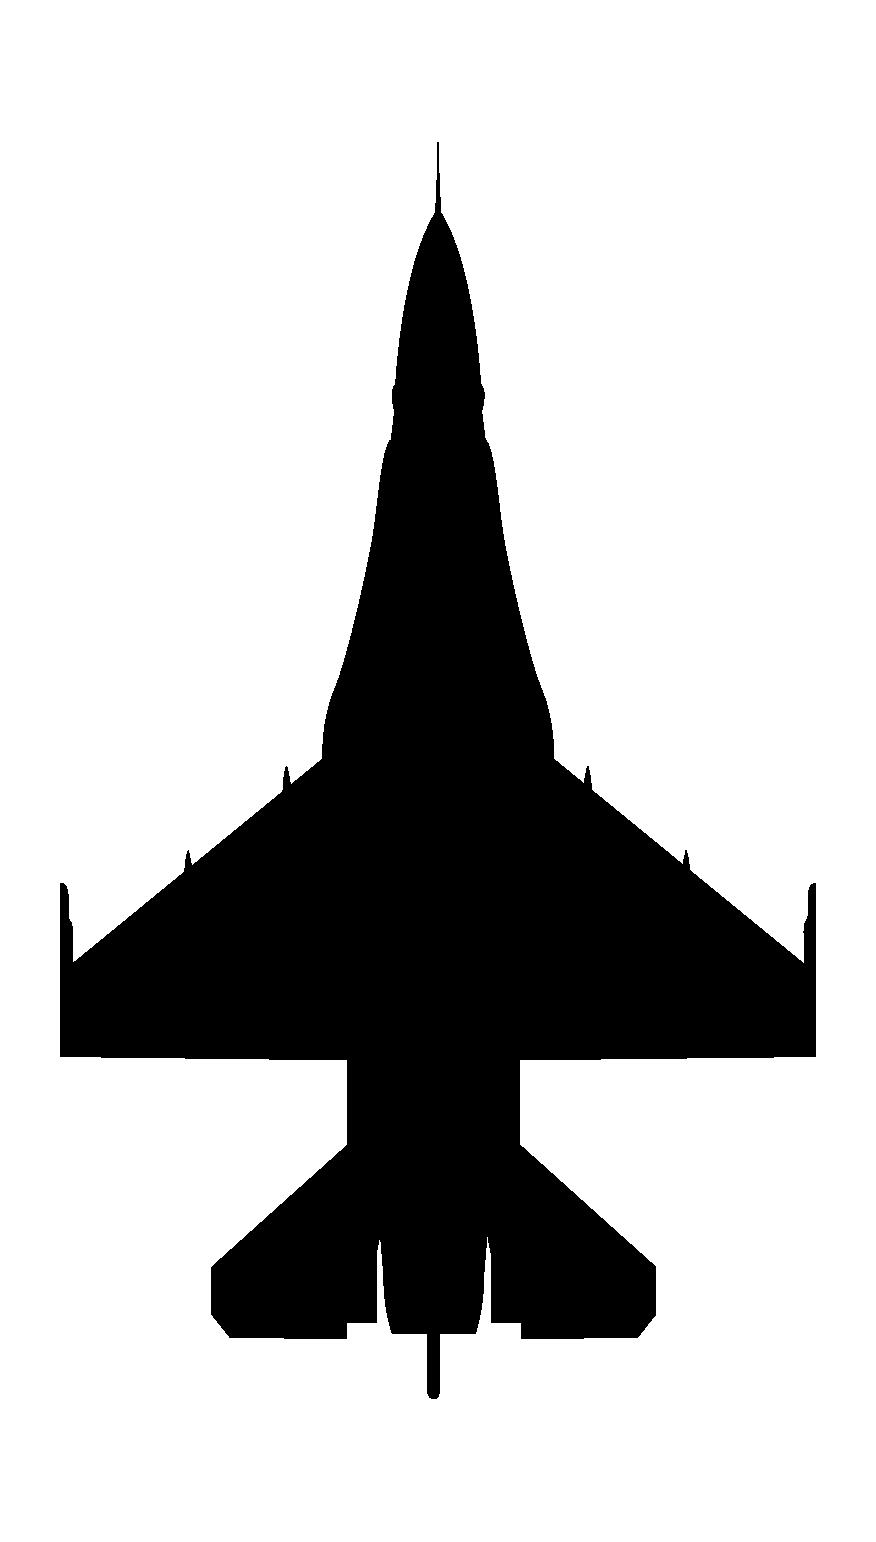
\includegraphics[
                    width=7.5mm,
                ]{diagrams/aircraft/silhouette_f16_top.pdf}
            };
            
            \node[yshift=-2mm] (2fig) at (2) {
                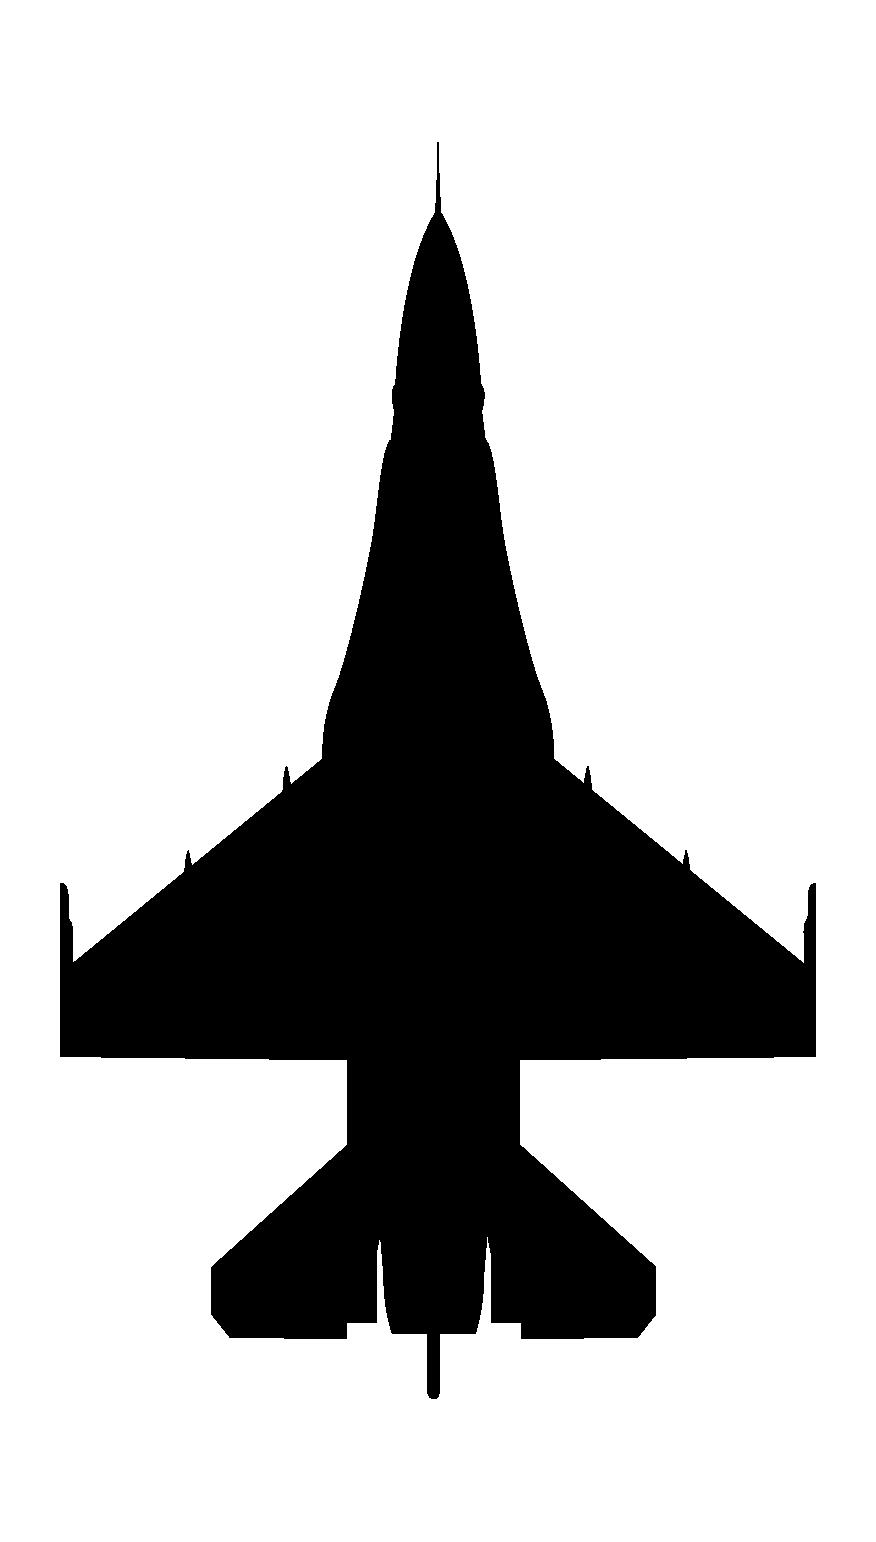
\includegraphics[
                    width=7.5mm,
                ]{diagrams/aircraft/silhouette_f16_top.pdf}
            };

            \node[yshift=-2mm] (3fig) at (3) {
                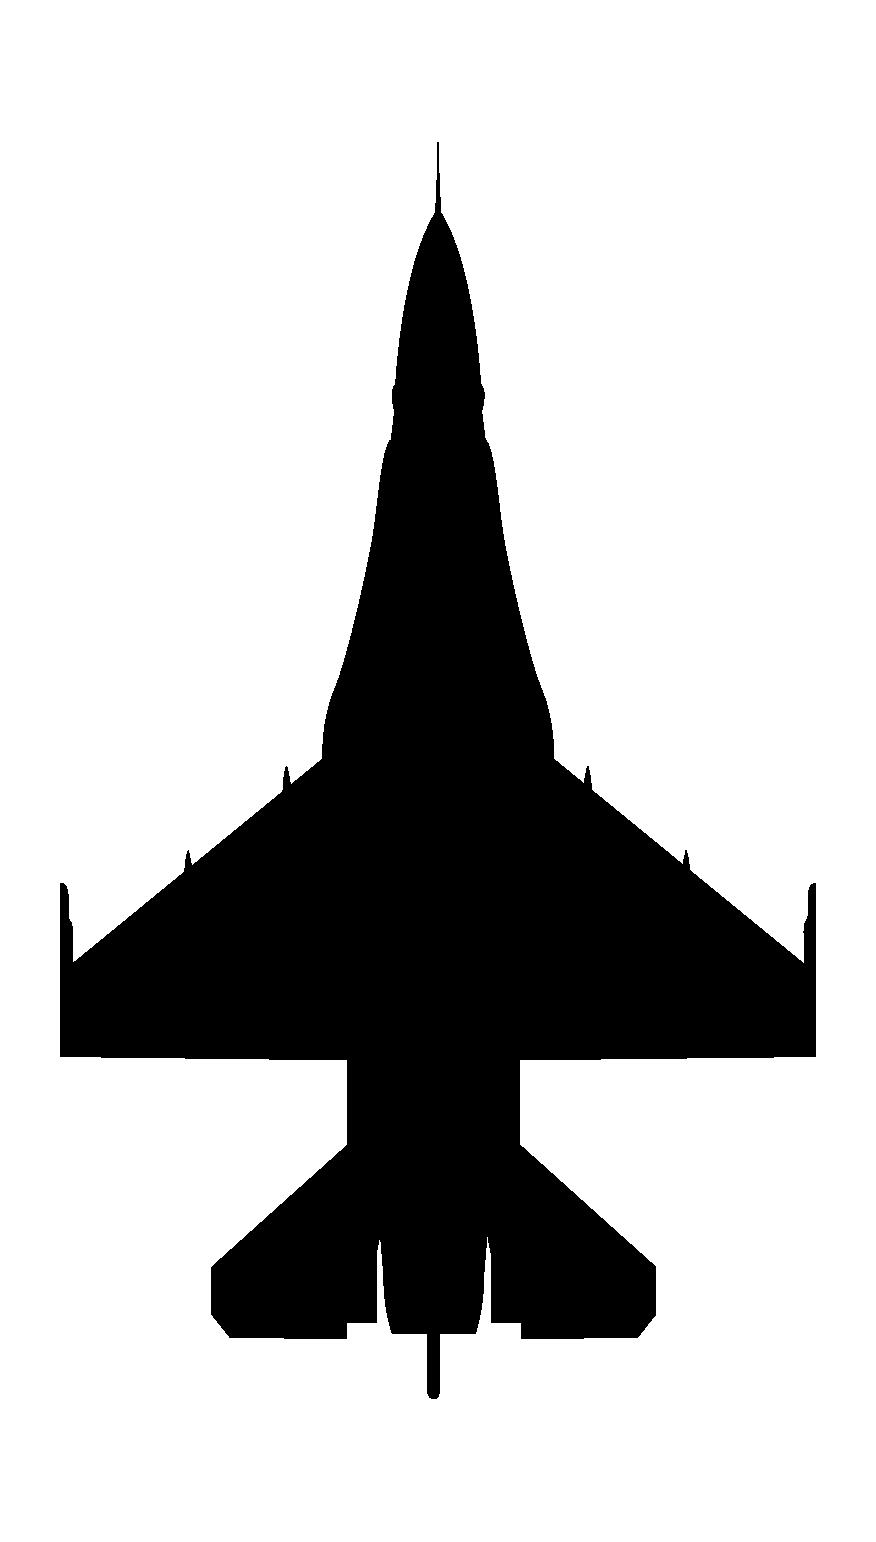
\includegraphics[
                    width=7.5mm,
                ]{diagrams/aircraft/silhouette_f16_top.pdf}
            };
            
            \node[yshift=-2mm] (4fig) at (4) {
                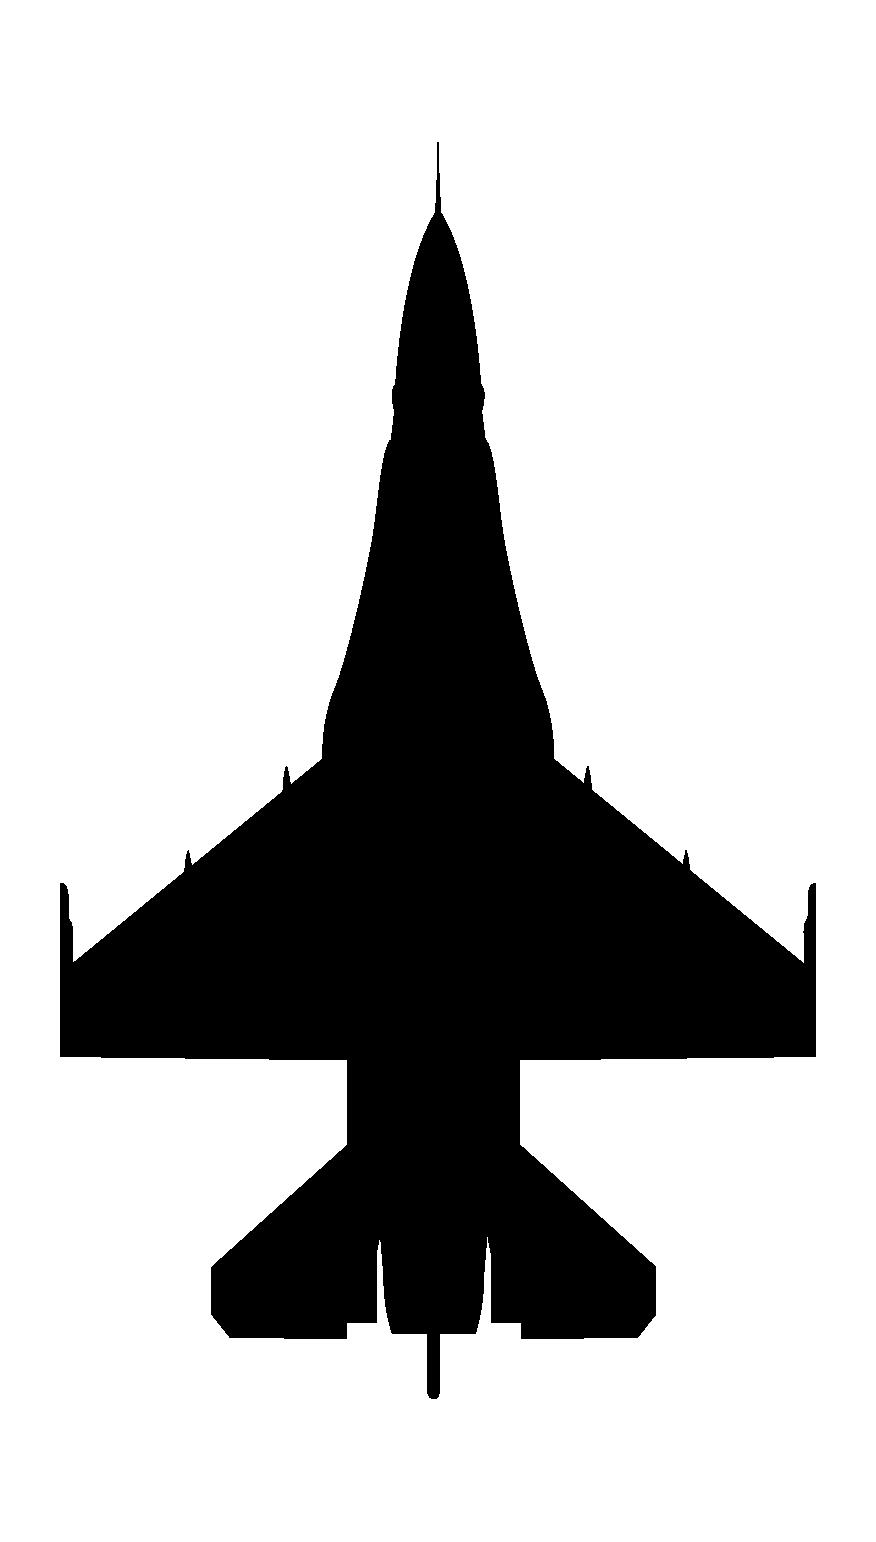
\includegraphics[
                    width=7.5mm,
                ]{diagrams/aircraft/silhouette_f16_top.pdf}
            };

            \node[anchor=north, font=\footnotesize] (1label) at (1fig.south) {1};
            \node[anchor=north, font=\footnotesize] (2label) at (2fig.south) {2};
            \node[anchor=north, font=\footnotesize] (3label) at (3fig.south) {3};
            \node[anchor=north, font=\footnotesize] (4label) at (4fig.south) {4};

        \end{tikzpicture}
        \caption{Four-ship offset box formation}
        \label{fig:supp_fig:form:boxoffset}
    \end{minipage}
\end{figure}

\begin{figure}[htbp]
    \centering
    \begin{tikzpicture}[figstyle]
        
        \coordinate (1) at (0,0);
        \coordinate (2) at ($(1)+(-135:20)$);
        \coordinate (3) at ($(1)+(20,0)$);
        \coordinate (4) at ($(3)+(-45:20)$);

        \draw[thin]
        (1) -- (2) node[font=\footnotesize, pos=0.5, above left] {fighting wing}
        (3) -- (4)node[font=\footnotesize, pos=0.5, above right] {fighting wing};

        \draw[thin, <->]
        ($(1)+(0,5)$) 
        -- ($(3)+(0,5)$)
        node[font=\footnotesize, pos=0.5, above] {line abreast};
        \draw[thin]
        (1) -- ($(1)+(0,7)$)
        (3) -- ($(3)+(0,7)$);

        \node[yshift=-2mm] (1fig) at (1) {
            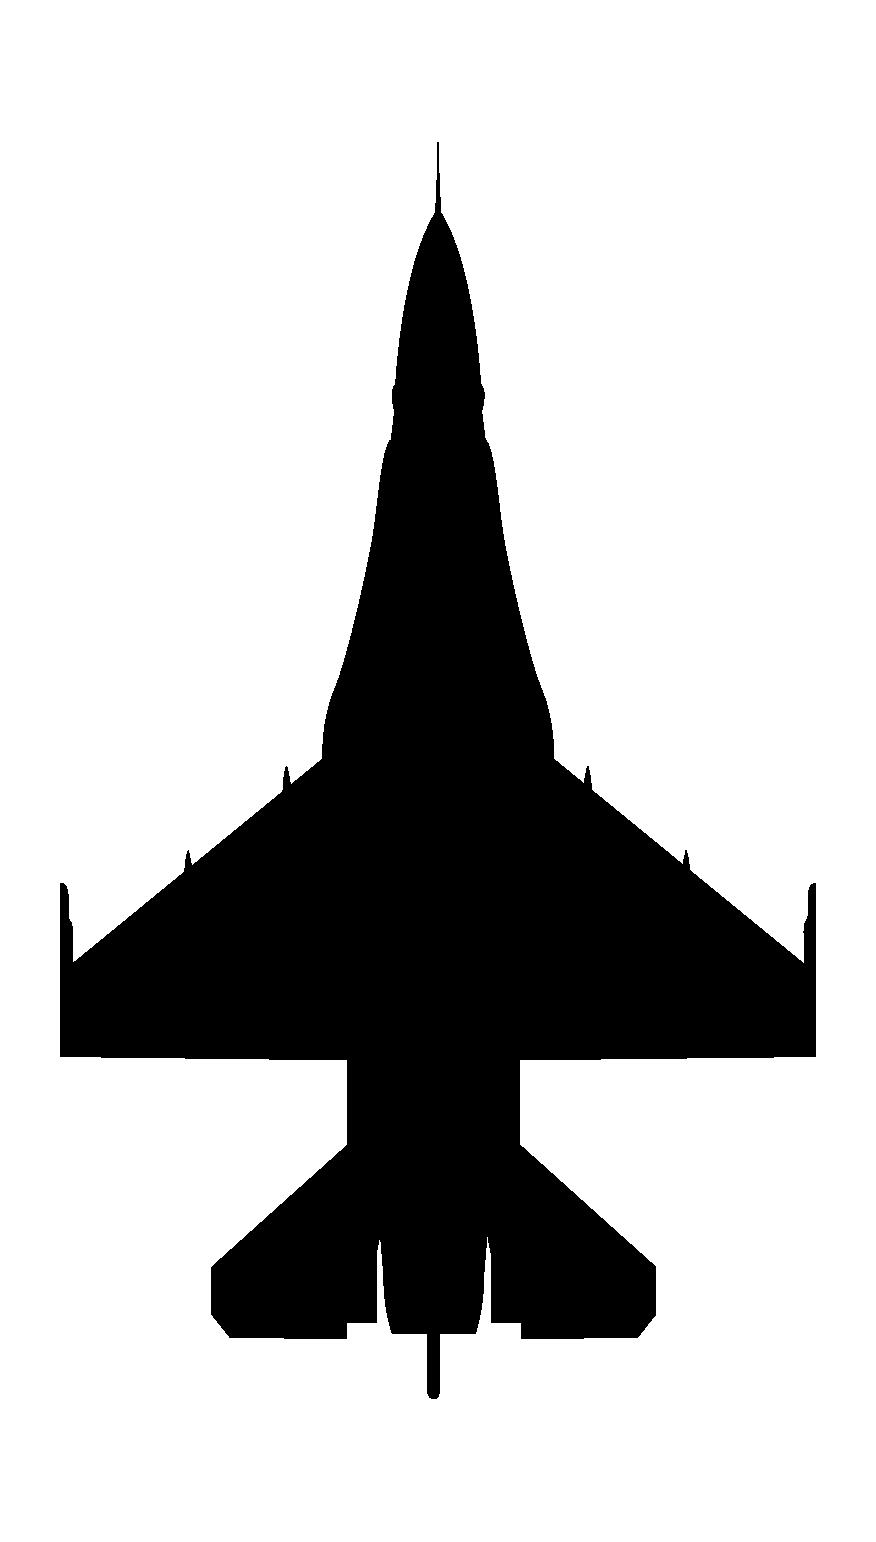
\includegraphics[
                width=7.5mm,
            ]{diagrams/aircraft/silhouette_f16_top.pdf}
        };
        
        \node[yshift=-2mm] (2fig) at (2) {
            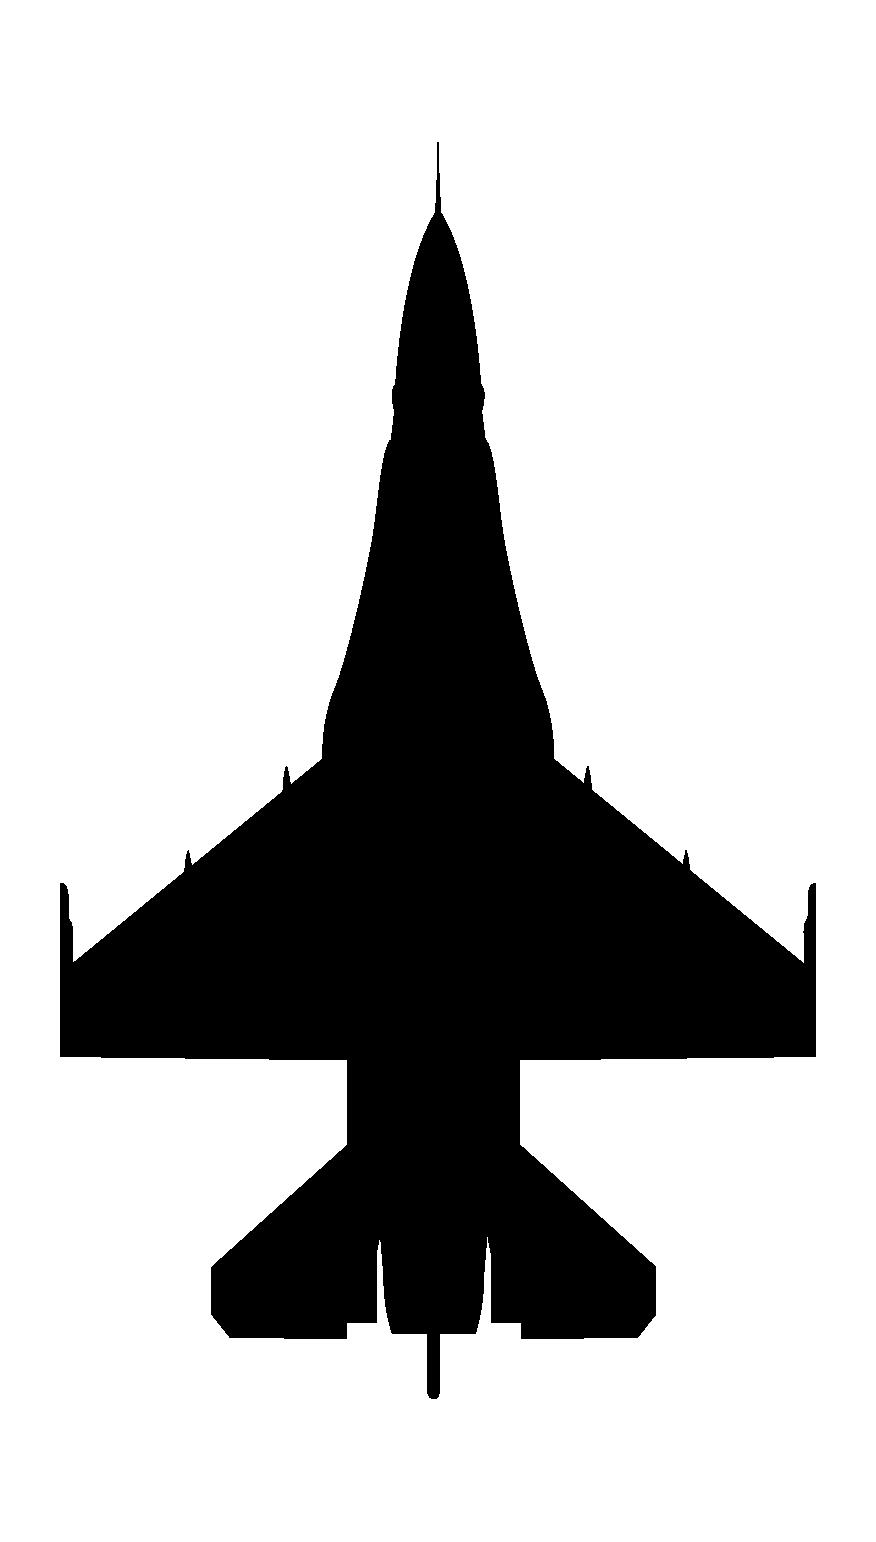
\includegraphics[
                width=7.5mm,
            ]{diagrams/aircraft/silhouette_f16_top.pdf}
        };

        \node[yshift=-2mm] (3fig) at (3) {
            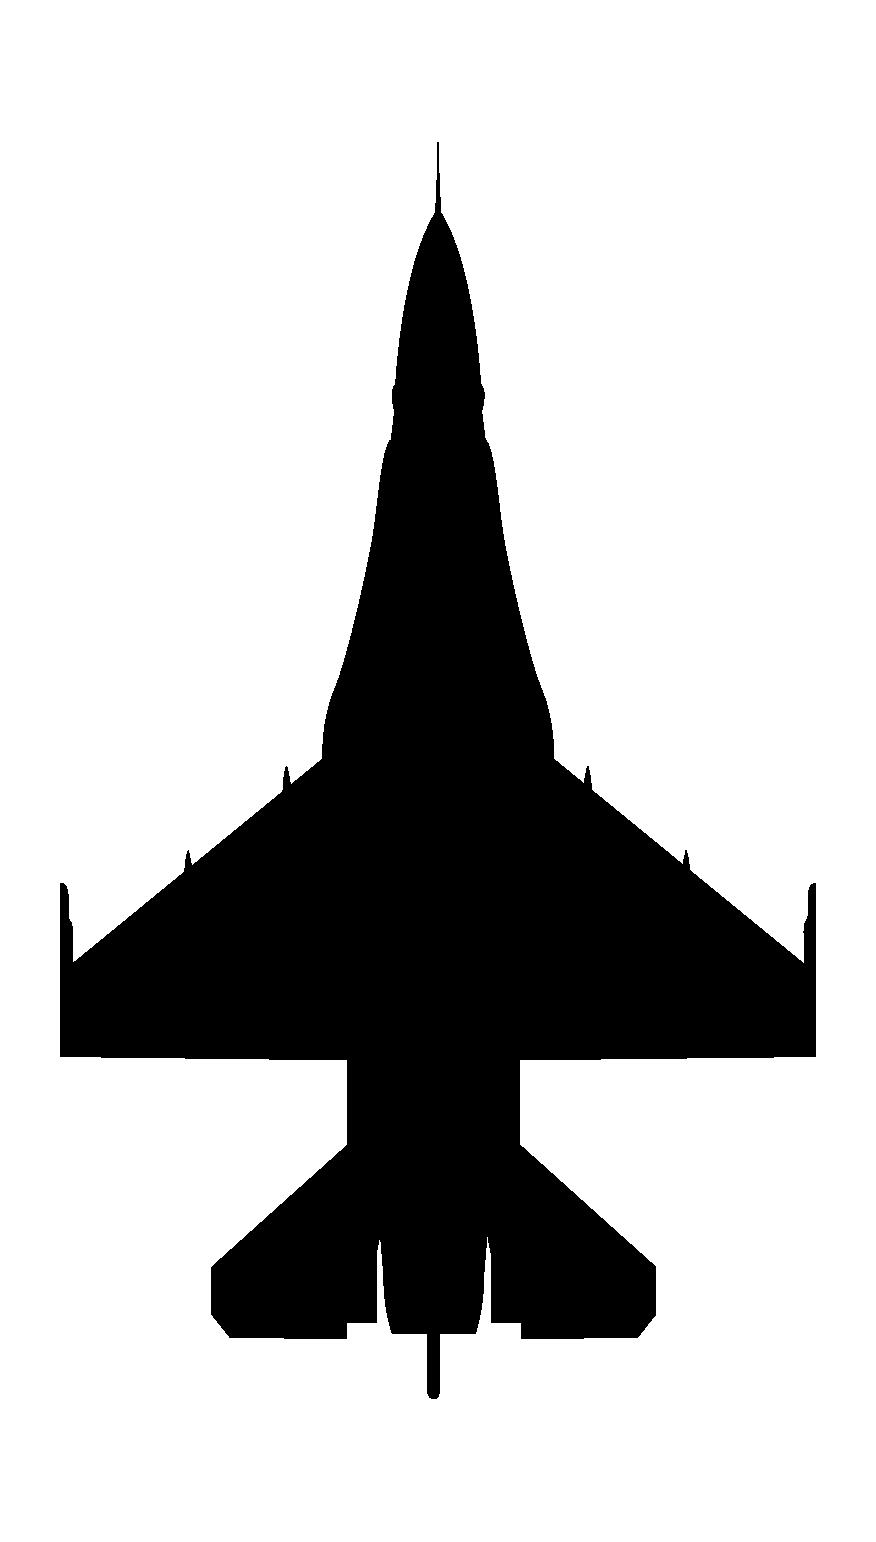
\includegraphics[
                width=7.5mm,
            ]{diagrams/aircraft/silhouette_f16_top.pdf}
        };
        
        \node[yshift=-2mm] (4fig) at (4) {
            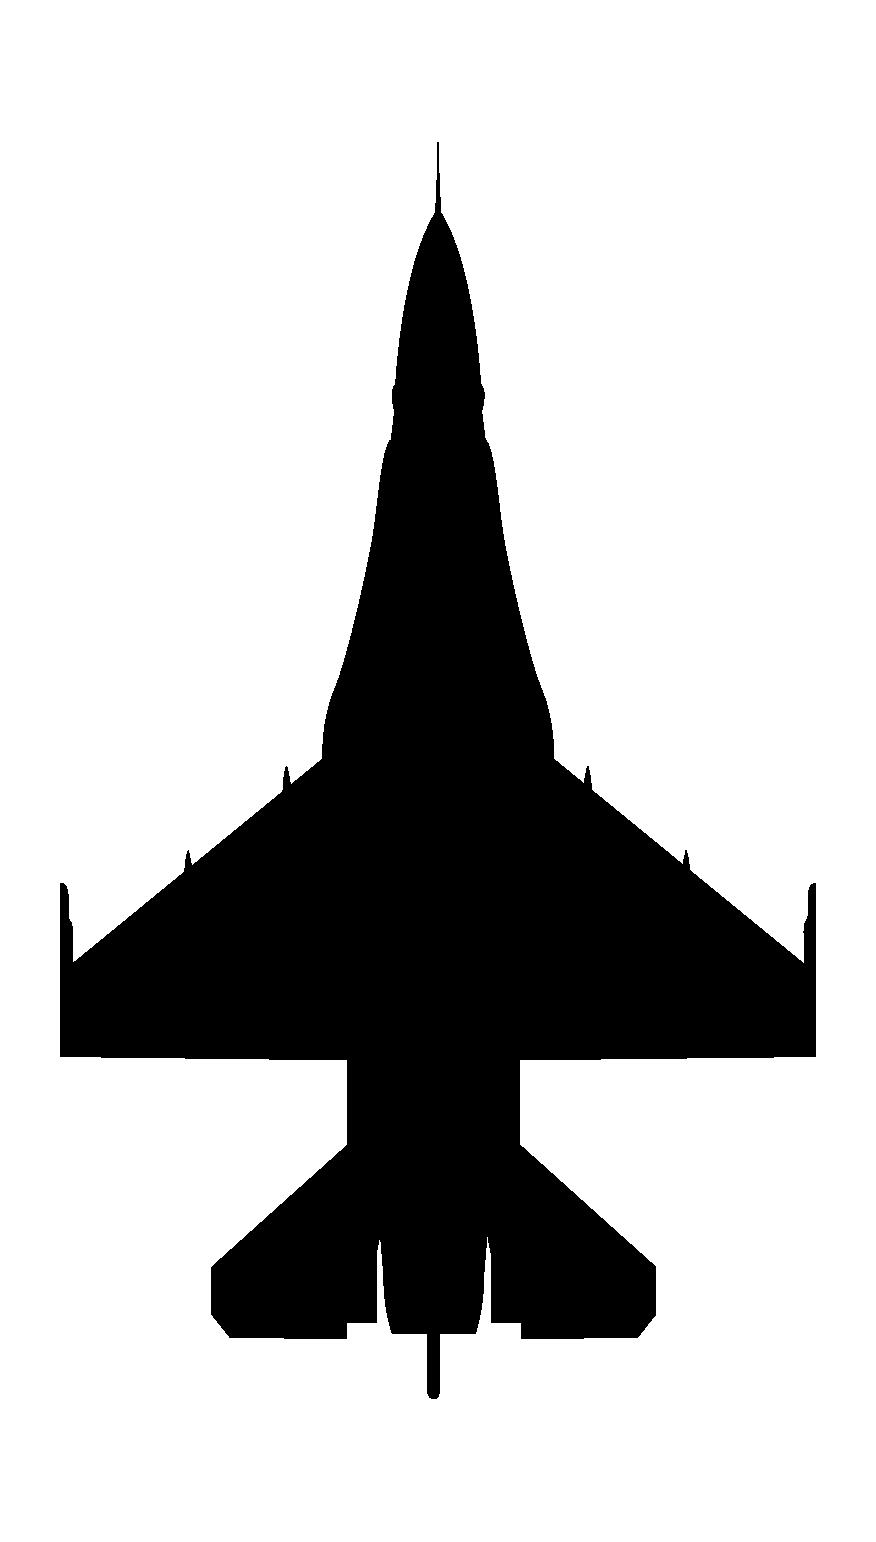
\includegraphics[
                width=7.5mm,
            ]{diagrams/aircraft/silhouette_f16_top.pdf}
        };

        \node[anchor=north, font=\footnotesize] (1label) at (1fig.south) {1};
        \node[anchor=north, font=\footnotesize] (2label) at (2fig.south) {2};
        \node[anchor=north, font=\footnotesize] (3label) at (3fig.south) {3};
        \node[anchor=north, font=\footnotesize] (4label) at (4fig.south) {4};

    \end{tikzpicture}
    \caption{Fluid-four formation}
    \label{fig:supp_fig:form:fluidfour}
\end{figure}

\begin{figure}[htbp]
    \centering
    \begin{minipage}[b]{0.5\textwidth}
        \centering
        \begin{tikzpicture}[figstyle]
            
            \coordinate (1) at (0,0);
            \coordinate (2) at ($(1)+(-150:15)$);
            \coordinate (3) at ($(1)+(-30:15)$);
            \coordinate (4) at ($(3)+(-30:15)$);

            \node[yshift=-2mm] (1fig) at (1) {
                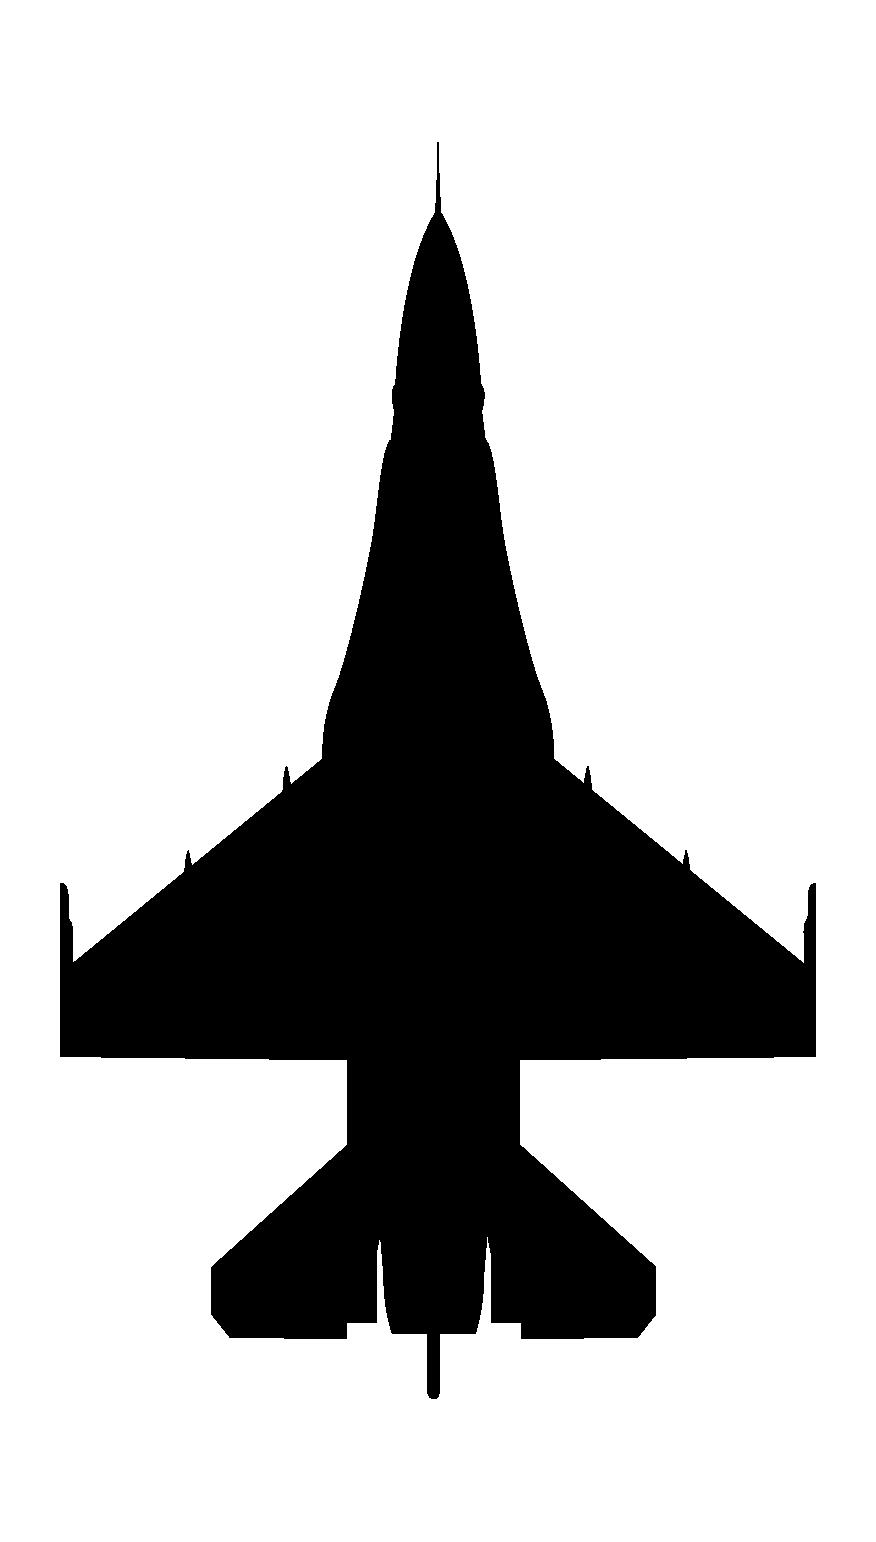
\includegraphics[
                    width=7.5mm,
                ]{diagrams/aircraft/silhouette_f16_top.pdf}
            };
            
            \node[yshift=-2mm] (2fig) at (2) {
                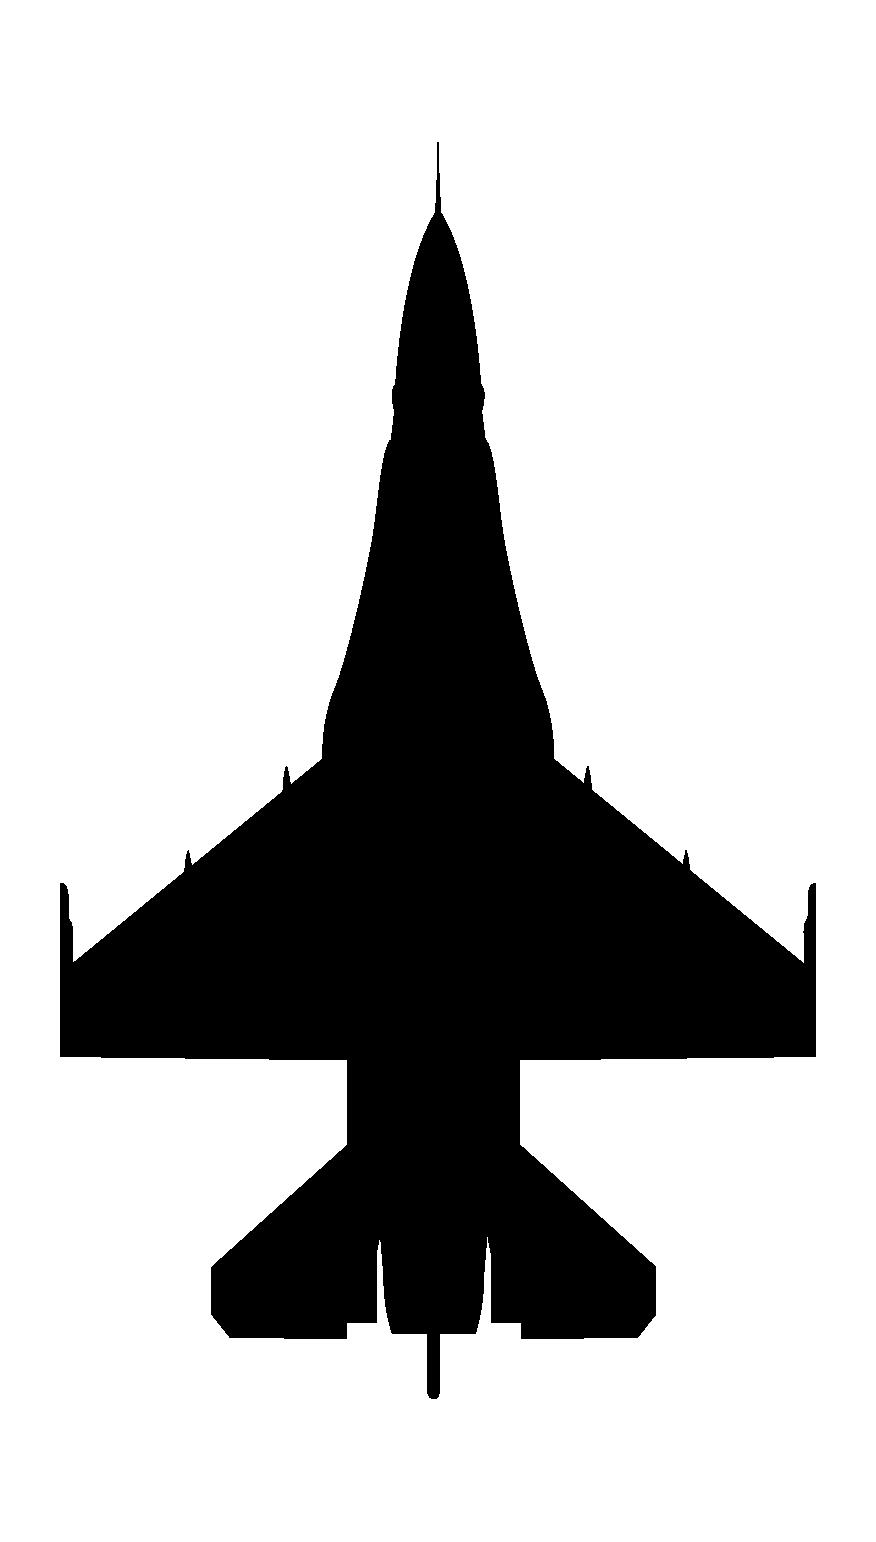
\includegraphics[
                    width=7.5mm,
                ]{diagrams/aircraft/silhouette_f16_top.pdf}
            };

            \node[yshift=-2mm] (3fig) at (3) {
                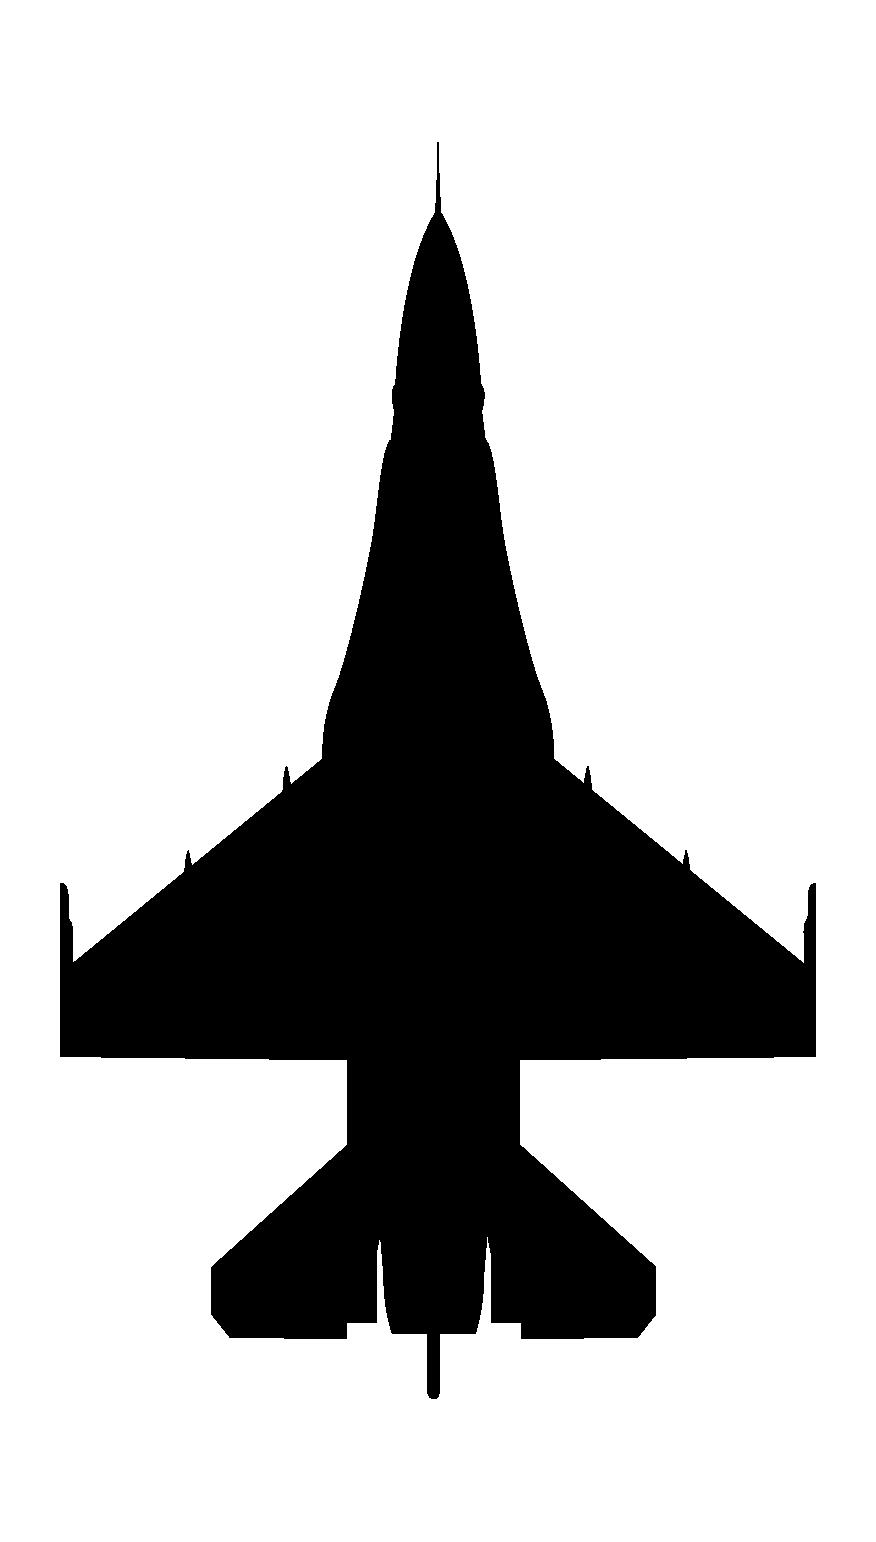
\includegraphics[
                    width=7.5mm,
                ]{diagrams/aircraft/silhouette_f16_top.pdf}
            };
            
            \node[yshift=-2mm] (4fig) at (4) {
                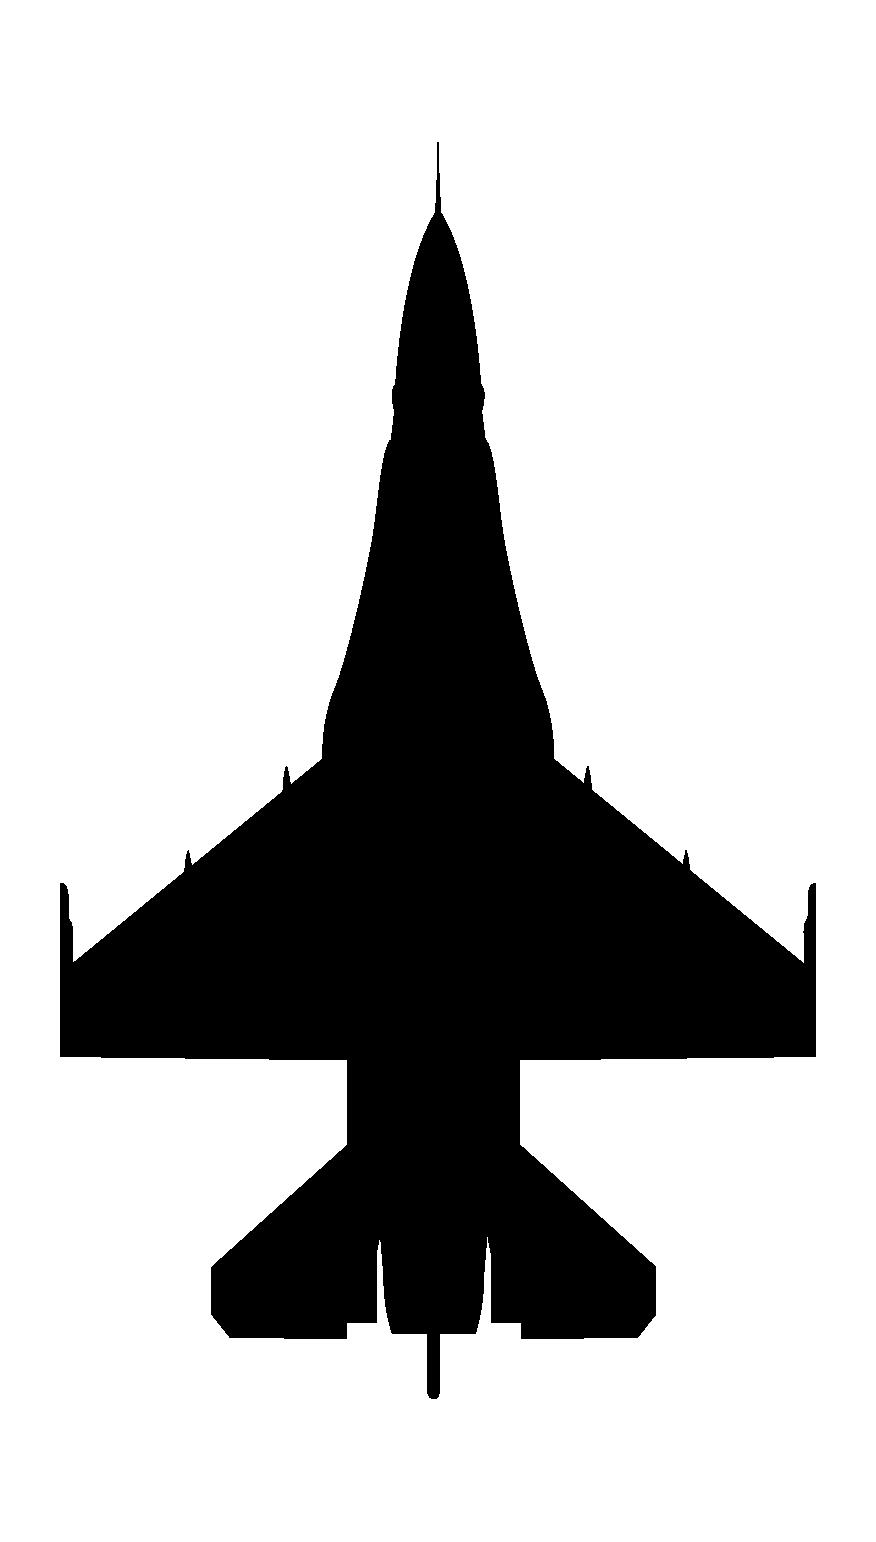
\includegraphics[
                    width=7.5mm,
                ]{diagrams/aircraft/silhouette_f16_top.pdf}
            };

            \node[anchor=north, font=\footnotesize] (1label) at (1fig.south) {1};
            \node[anchor=north, font=\footnotesize] (2label) at (2fig.south) {2};
            \node[anchor=north, font=\footnotesize] (3label) at (3fig.south) {3};
            \node[anchor=north, font=\footnotesize] (4label) at (4fig.south) {4};

        \end{tikzpicture}
        \caption{Fingertip formation}
        \label{fig:supp_fig:form:fingertip}
    \end{minipage}%
    \begin{minipage}[b]{0.5\textwidth}
        \centering
        \begin{tikzpicture}[figstyle]
            
            \coordinate (1) at (0,0);
            \coordinate (2) at ($(1)+(-150:20)$);
            \coordinate (3) at ($(1)+(-30:20)$);
            \coordinate (4) at ($(3)+(-150:20)$);

            \node[yshift=-2mm] (1fig) at (1) {
                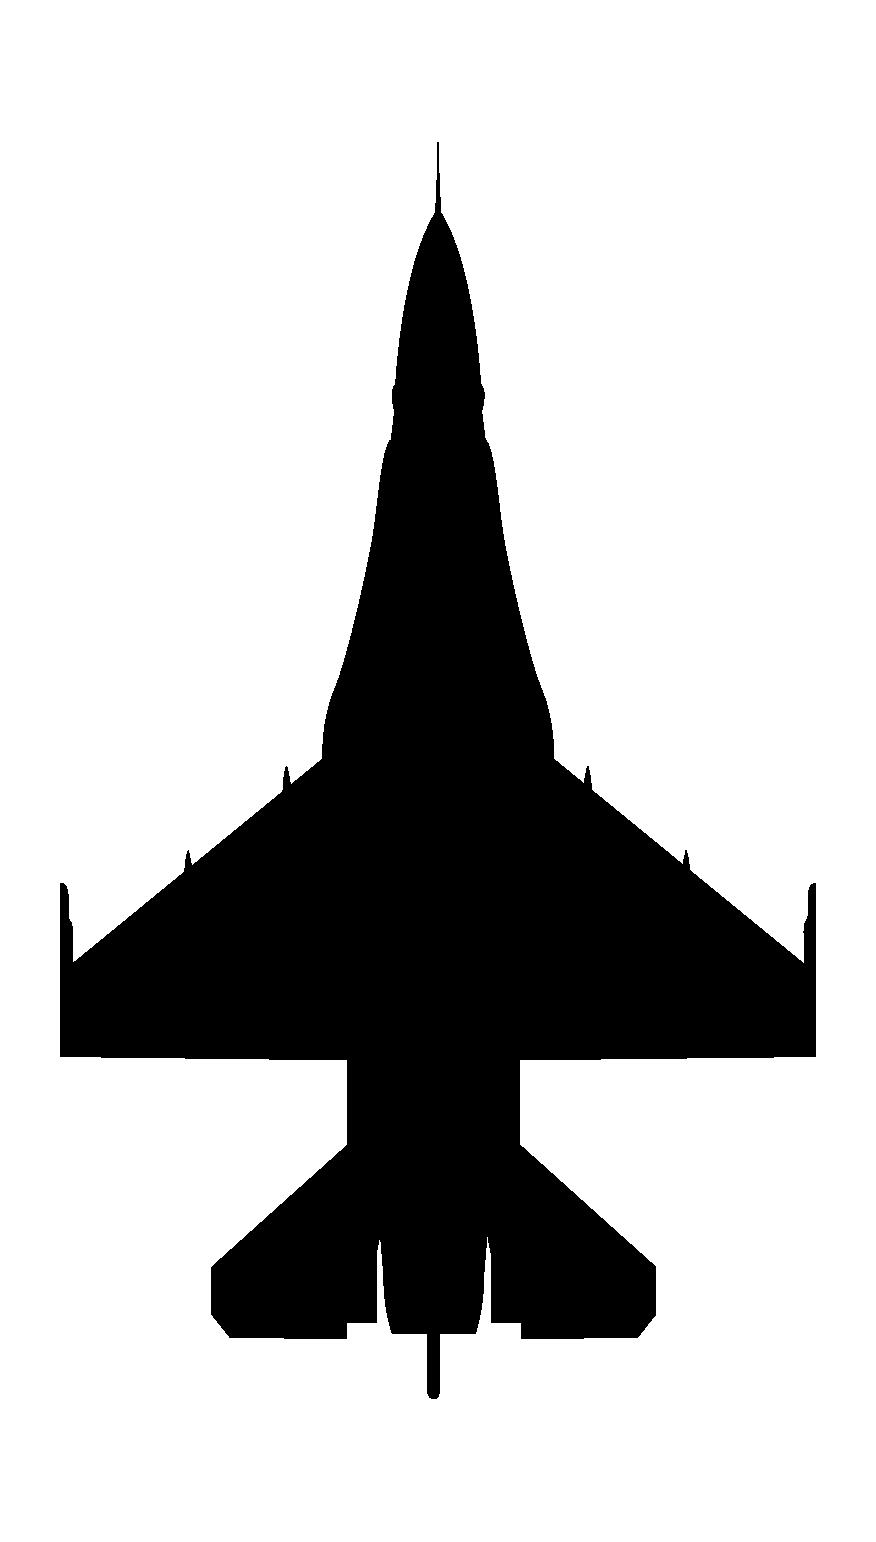
\includegraphics[
                    width=7.5mm,
                ]{diagrams/aircraft/silhouette_f16_top.pdf}
            };
            
            \node[yshift=-2mm] (2fig) at (2) {
                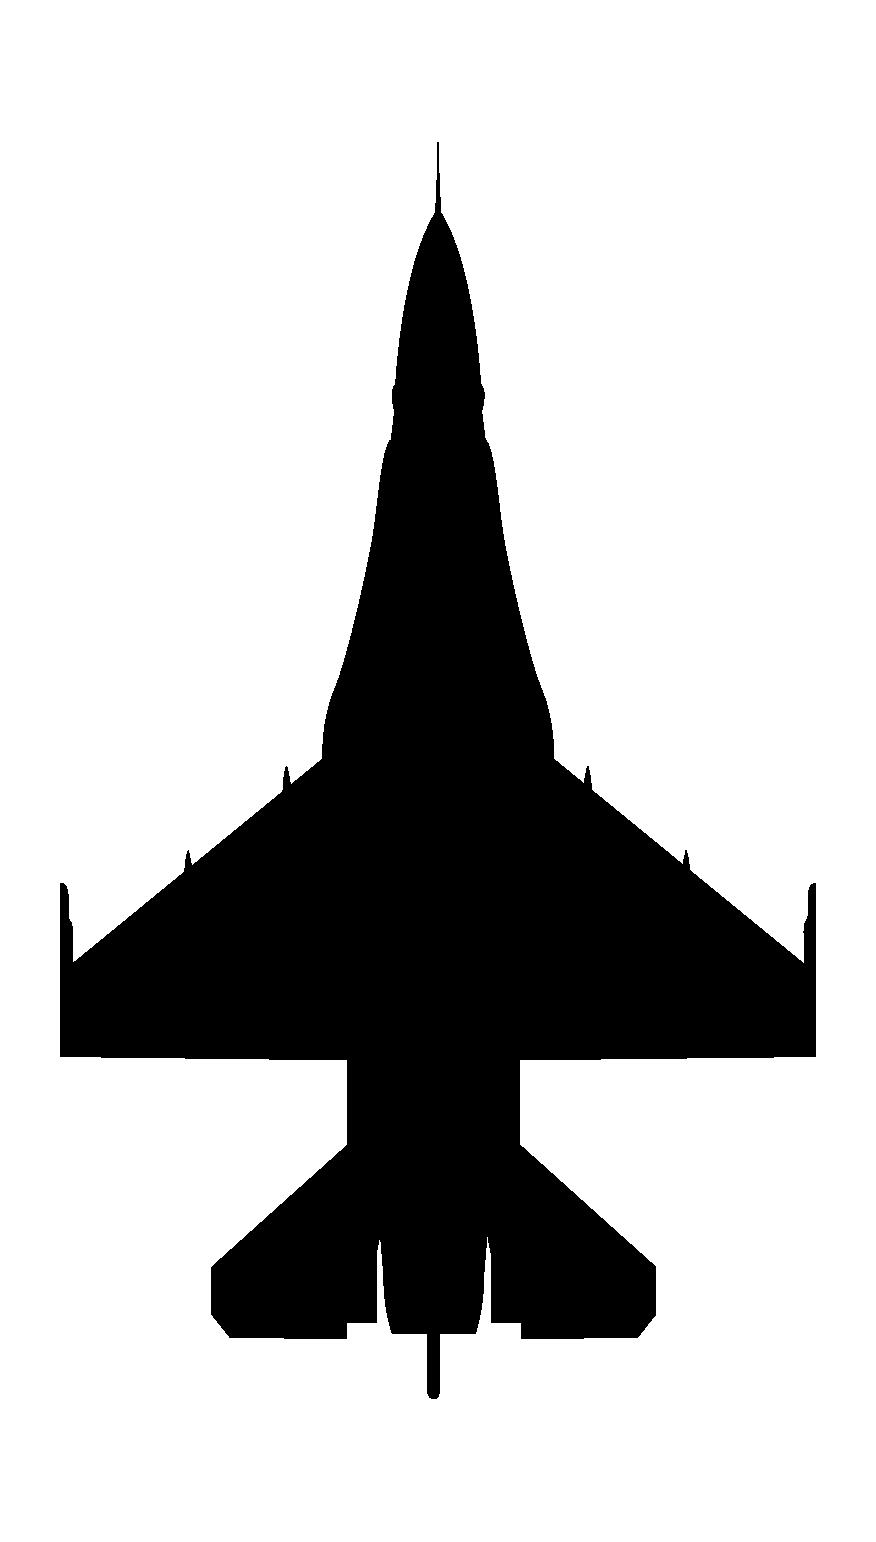
\includegraphics[
                    width=7.5mm,
                ]{diagrams/aircraft/silhouette_f16_top.pdf}
            };

            \node[yshift=-2mm] (3fig) at (3) {
                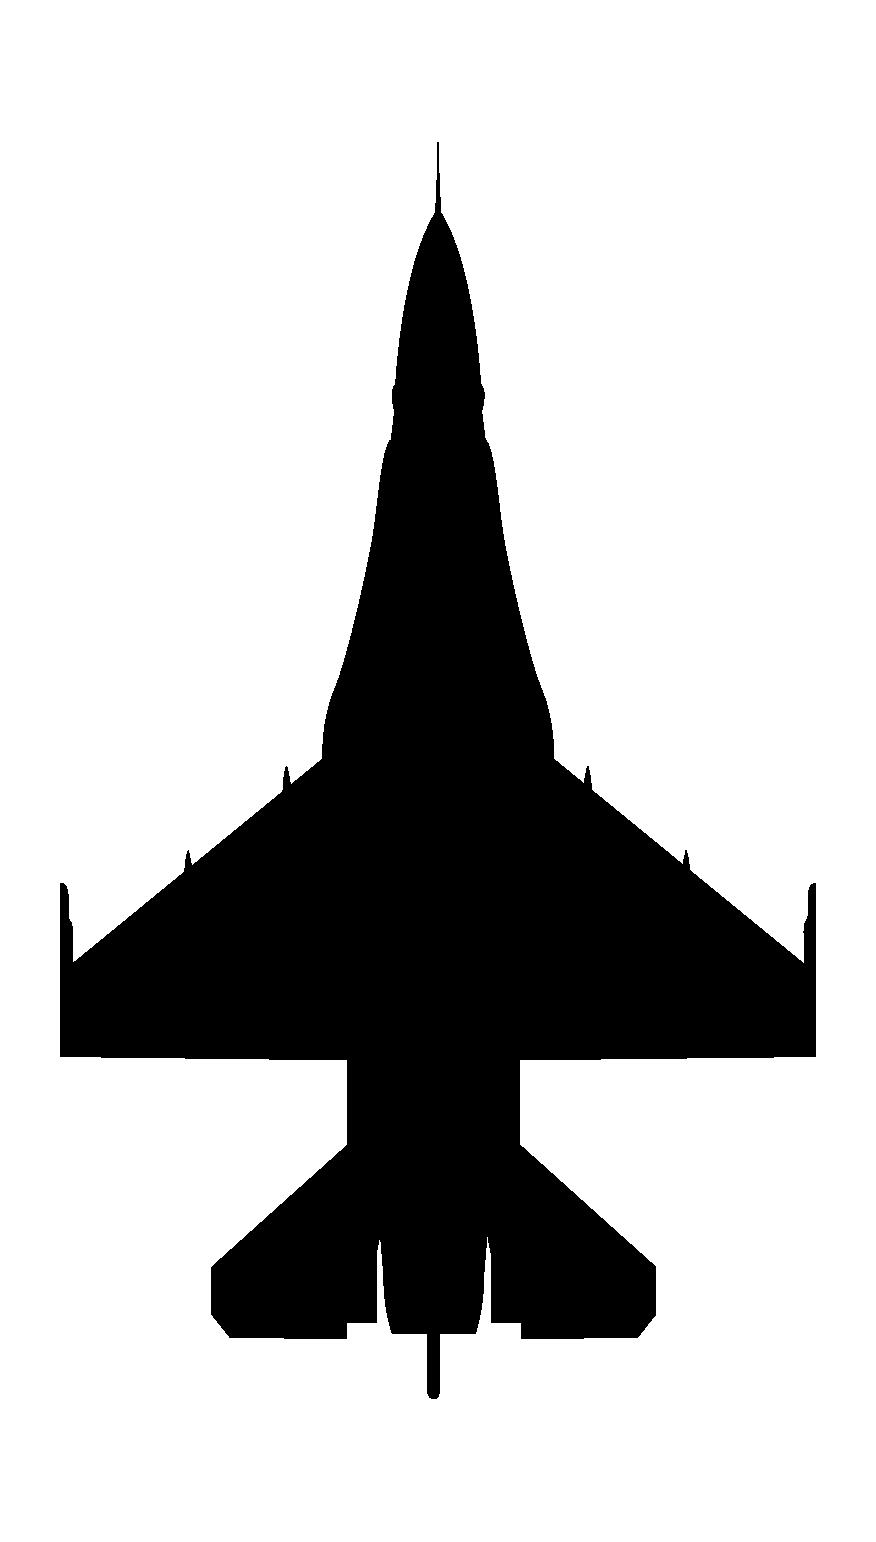
\includegraphics[
                    width=7.5mm,
                ]{diagrams/aircraft/silhouette_f16_top.pdf}
            };
            
            \node[yshift=-2mm] (4fig) at (4) {
                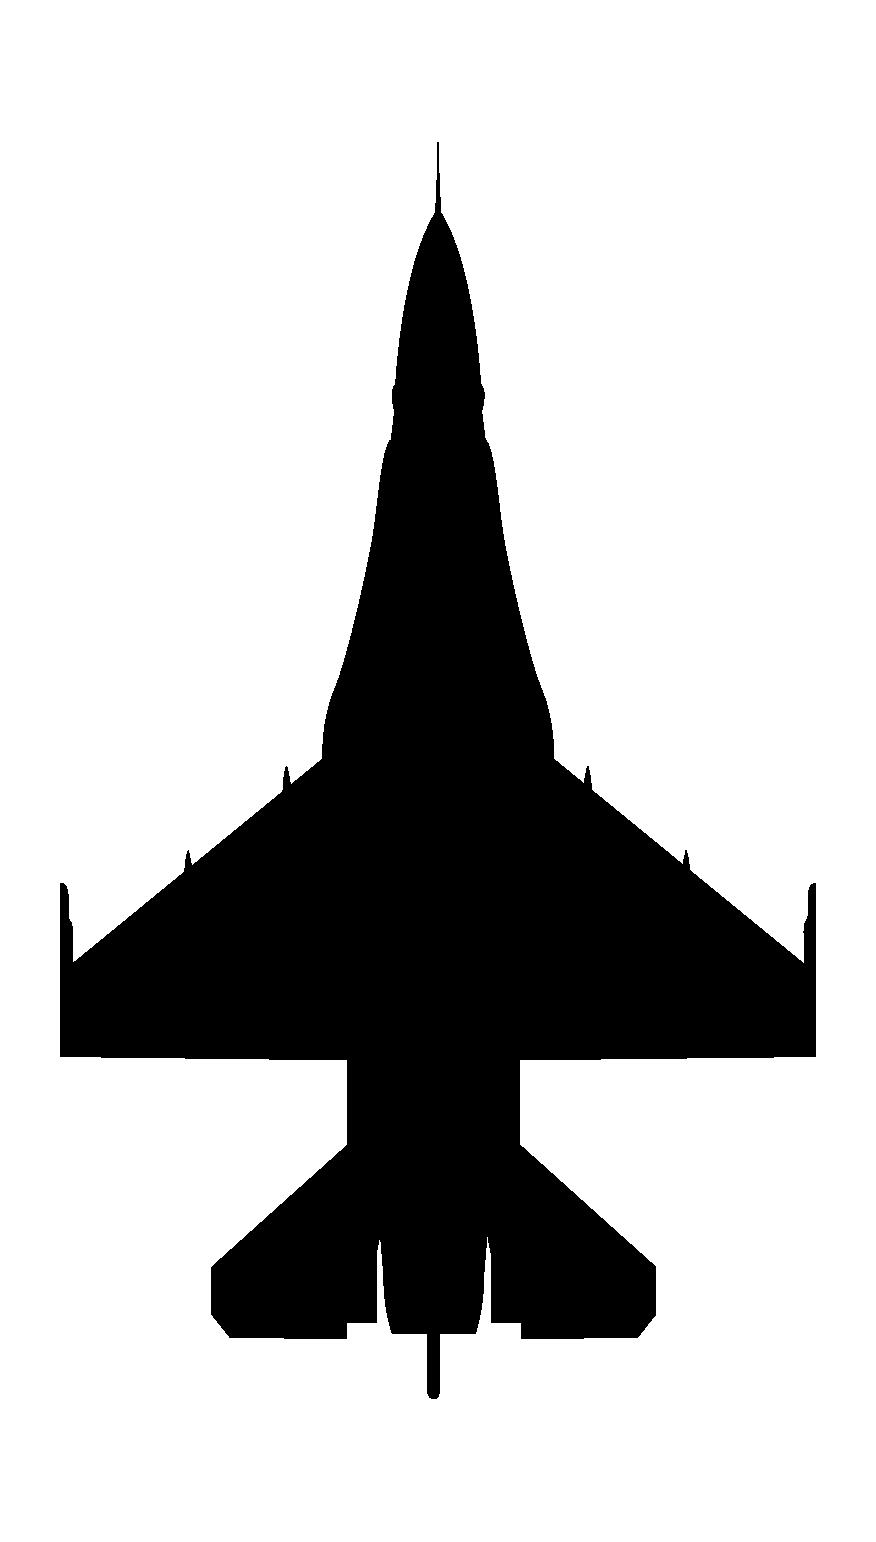
\includegraphics[
                    width=7.5mm,
                ]{diagrams/aircraft/silhouette_f16_top.pdf}
            };

            \node[anchor=north, font=\footnotesize] (1label) at (1fig.south) {1};
            \node[anchor=north, font=\footnotesize] (2label) at (2fig.south) {2};
            \node[anchor=north, font=\footnotesize] (3label) at (3fig.south) {3};
            \node[anchor=north, font=\footnotesize] (4label) at (4fig.south) {4};

        \end{tikzpicture}
        \caption{Diamond formation}
        \label{fig:supp_fig:form:diamond}
    \end{minipage}
\end{figure}

\begin{figure}[htbp]
    \centering
    \begin{minipage}[b]{0.5\textwidth}
        \centering
        \begin{tikzpicture}[figstyle]
            
            \coordinate (1) at (0,0);
            \coordinate (2) at ($(1)+(-90:15)$);
            \coordinate (3) at ($(2)+(-90:15)$);
            \coordinate (4) at ($(3)+(-90:15)$);

            \node[yshift=-2mm] (1fig) at (1) {
                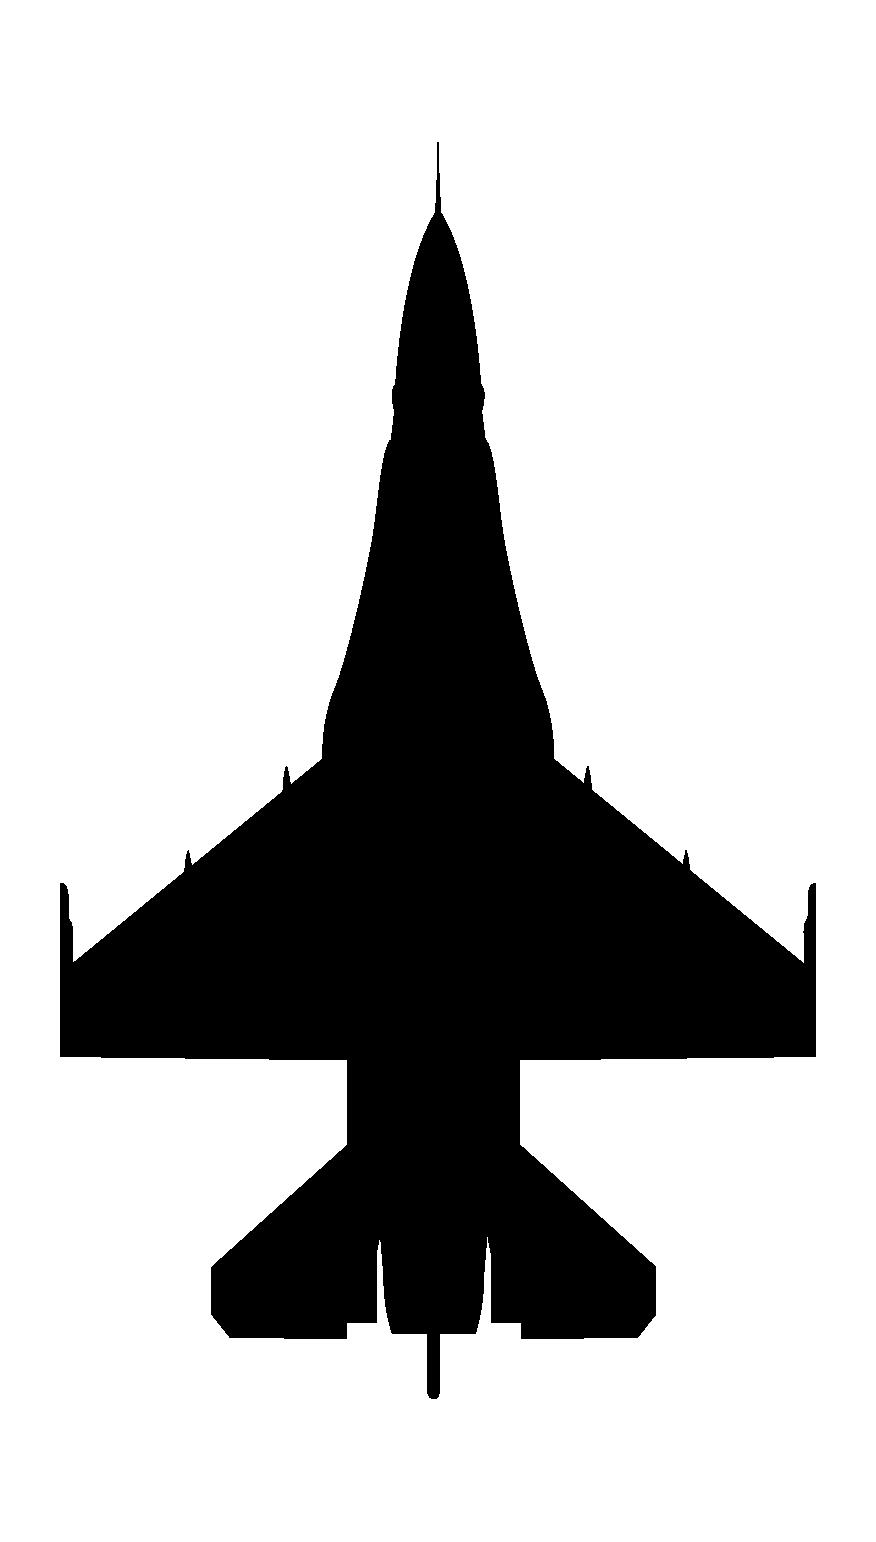
\includegraphics[
                    width=7.5mm,
                ]{diagrams/aircraft/silhouette_f16_top.pdf}
            };
            
            \node[yshift=-2mm] (2fig) at (2) {
                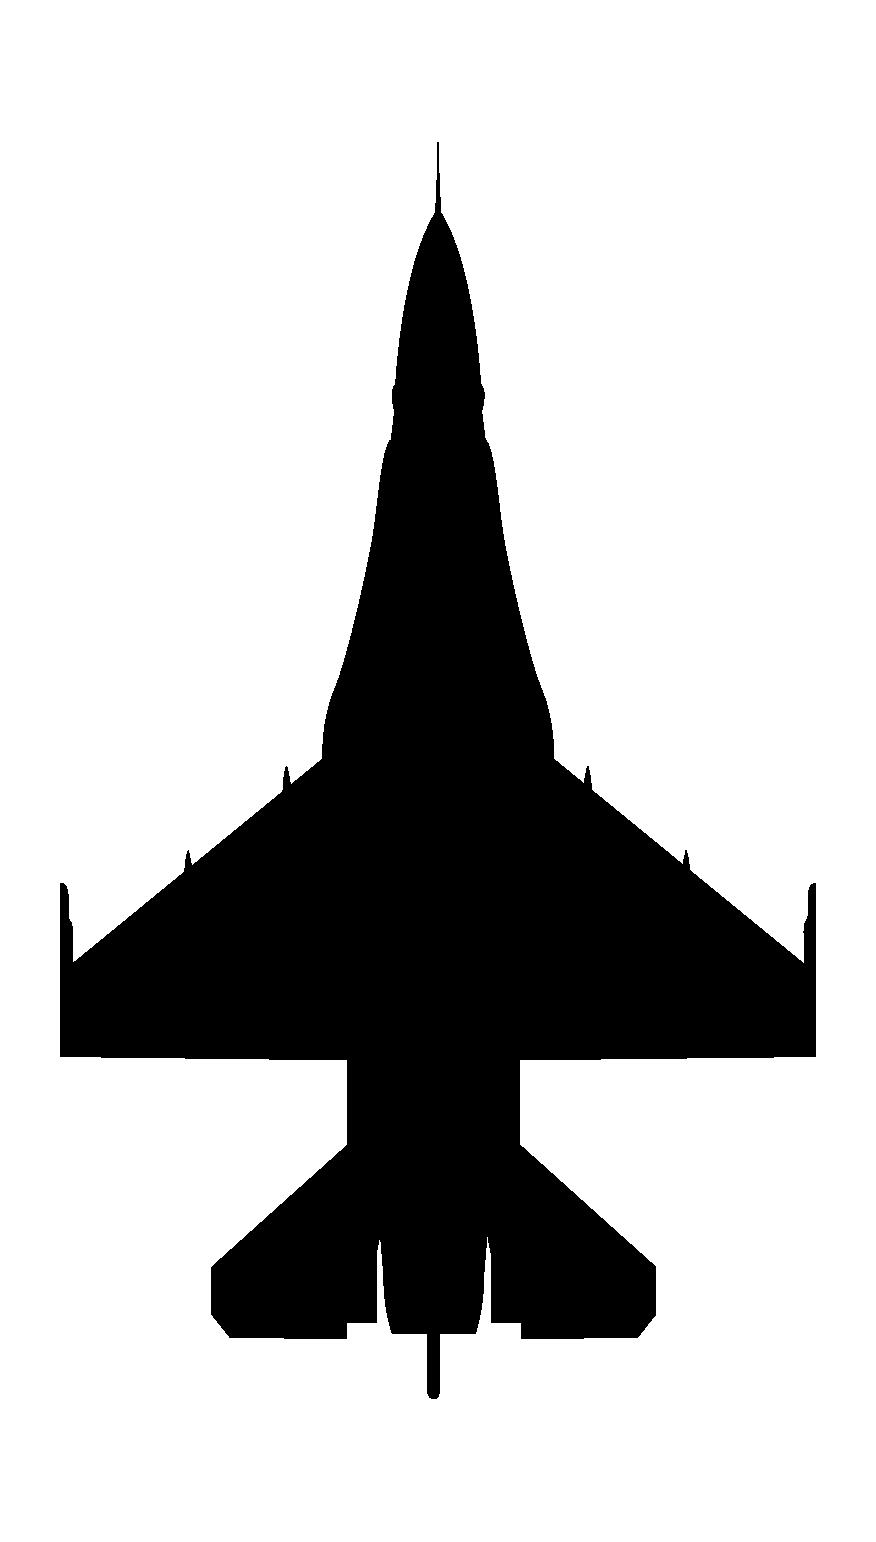
\includegraphics[
                    width=7.5mm,
                ]{diagrams/aircraft/silhouette_f16_top.pdf}
            };

            \node[yshift=-2mm] (3fig) at (3) {
                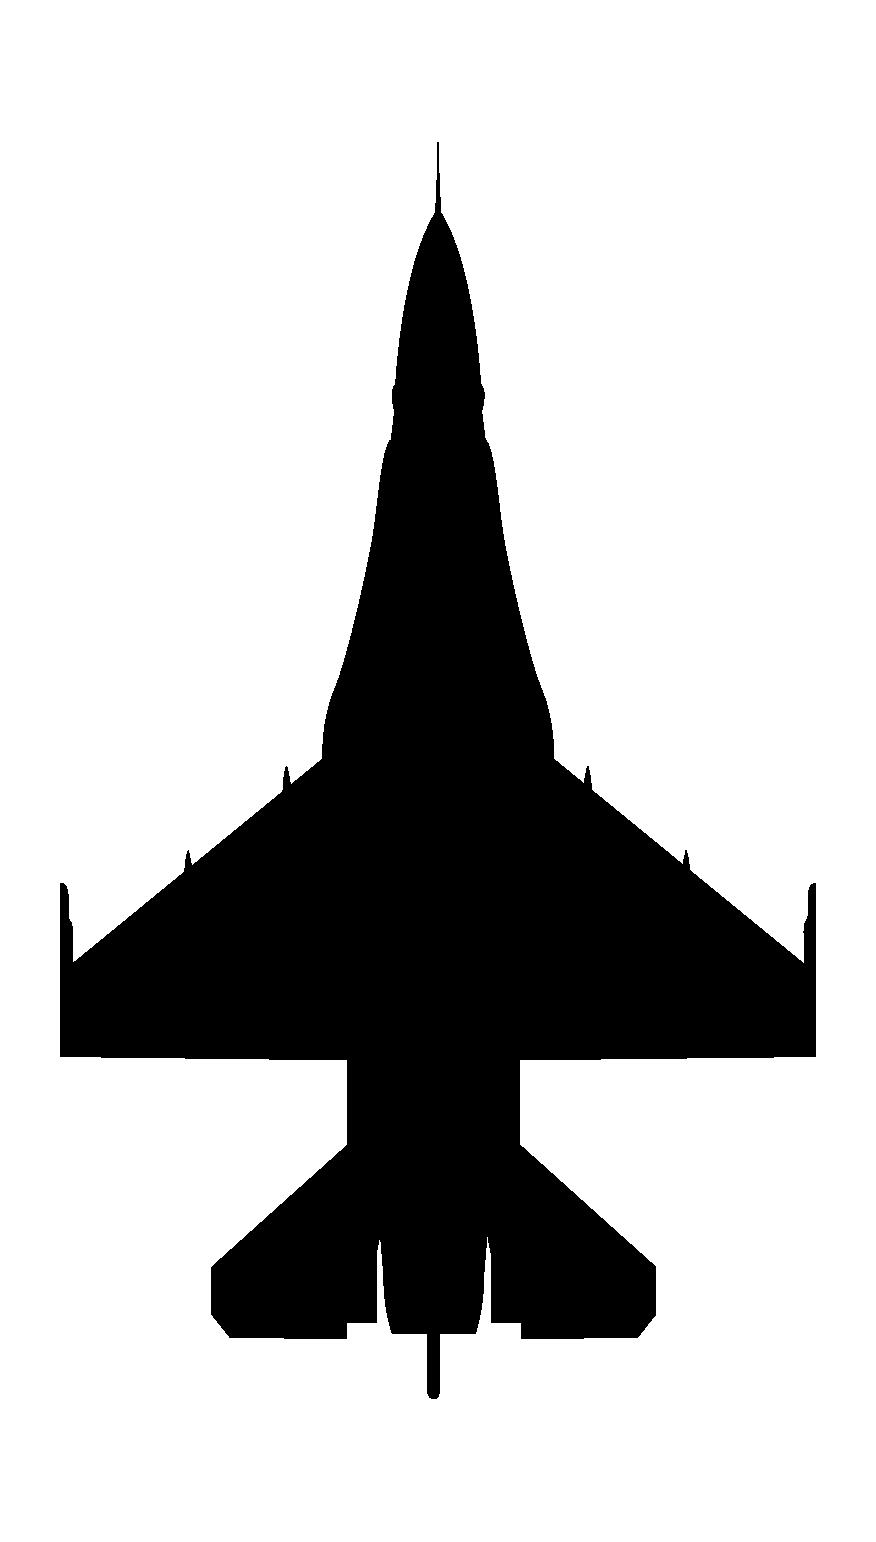
\includegraphics[
                    width=7.5mm,
                ]{diagrams/aircraft/silhouette_f16_top.pdf}
            };
            
            \node[yshift=-2mm] (4fig) at (4) {
                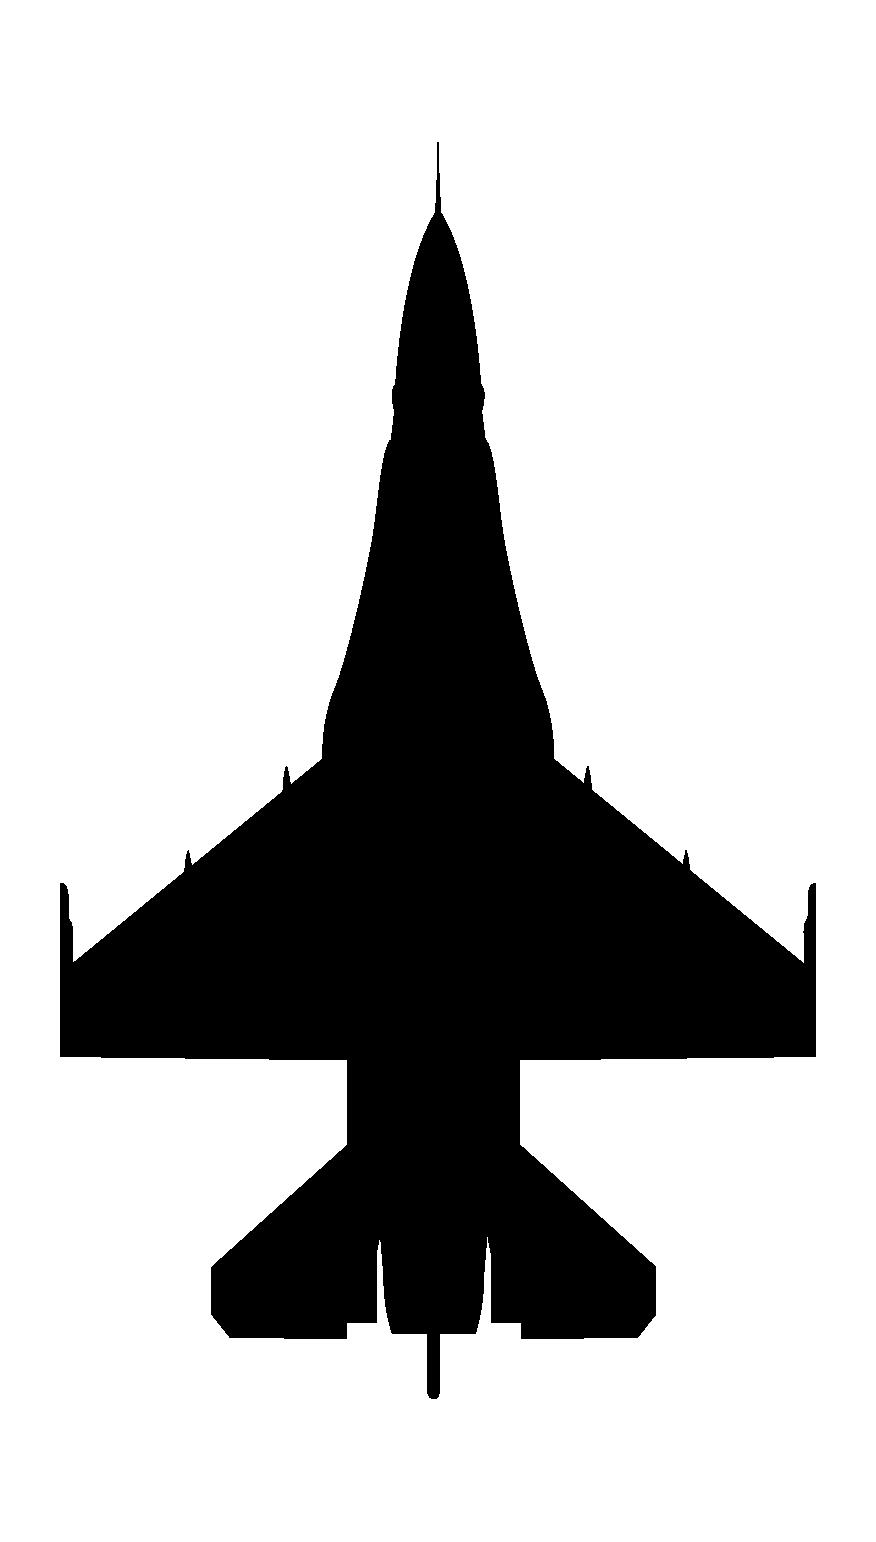
\includegraphics[
                    width=7.5mm,
                ]{diagrams/aircraft/silhouette_f16_top.pdf}
            };

            \node[anchor=west, font=\footnotesize] (1label) at (1fig.east) {1};
            \node[anchor=west, font=\footnotesize] (2label) at (2fig.east) {2};
            \node[anchor=west, font=\footnotesize] (3label) at (3fig.east) {3};
            \node[anchor=west, font=\footnotesize] (4label) at (4fig.east) {4};

        \end{tikzpicture}
        \caption{Trail formation}
        \label{fig:supp_fig:form:trail}
    \end{minipage}%
    \begin{minipage}[b]{0.5\textwidth}
        \centering
        \begin{tikzpicture}[figstyle]
            
            \coordinate (1) at (0,0);
            \coordinate (2) at ($(1)+(0:15)$);
            \coordinate (3) at ($(2)+(0:15)$);
            \coordinate (4) at ($(3)+(0:15)$);

            \node[yshift=-2mm] (1fig) at (1) {
                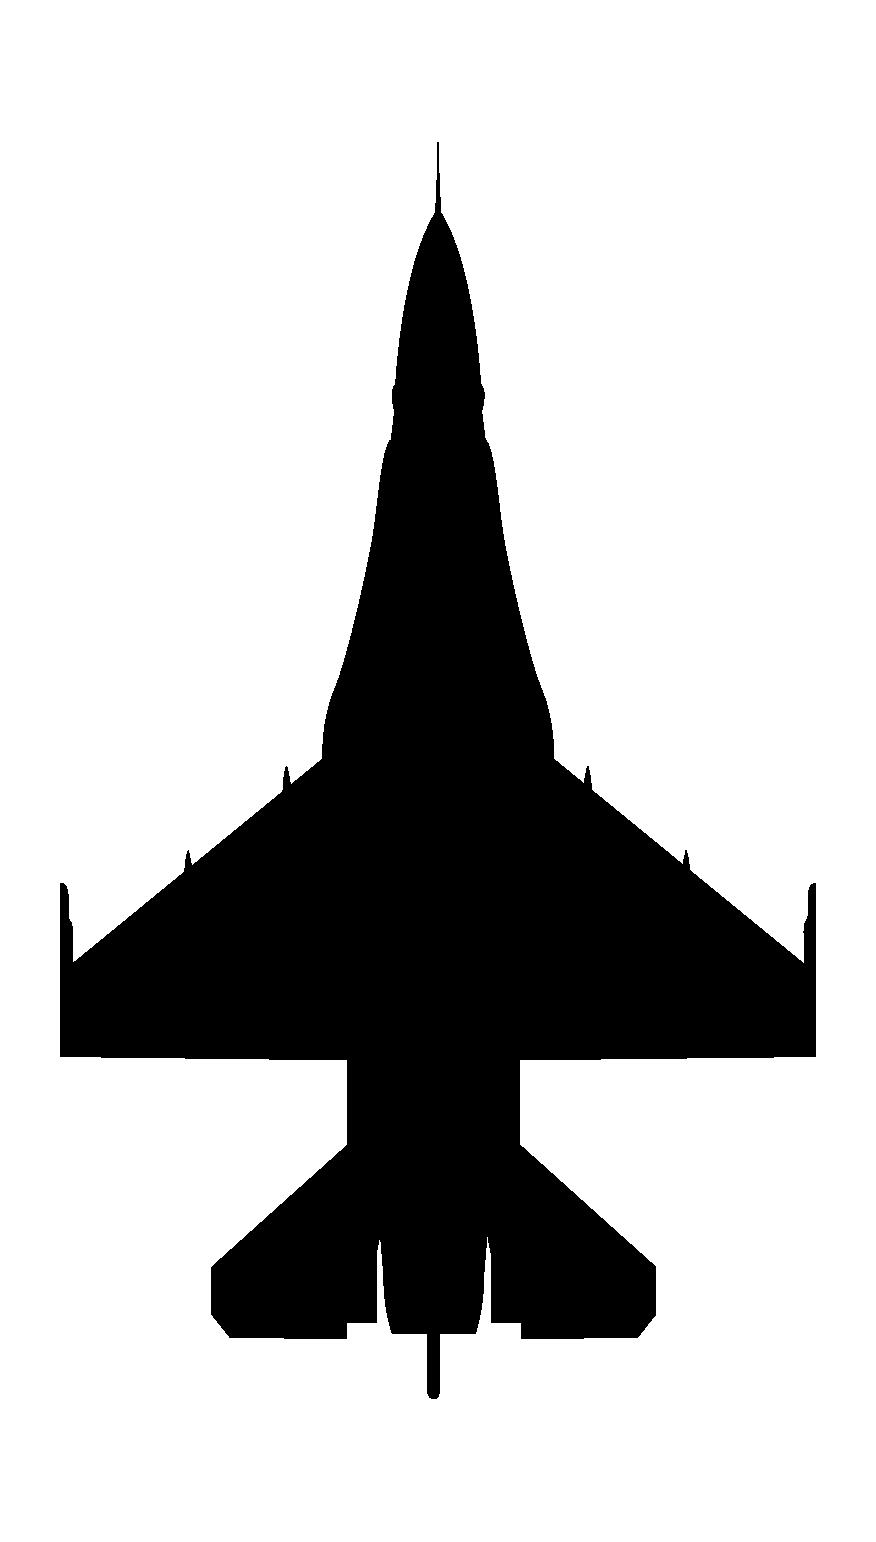
\includegraphics[
                    width=7.5mm,
                ]{diagrams/aircraft/silhouette_f16_top.pdf}
            };
            
            \node[yshift=-2mm] (2fig) at (2) {
                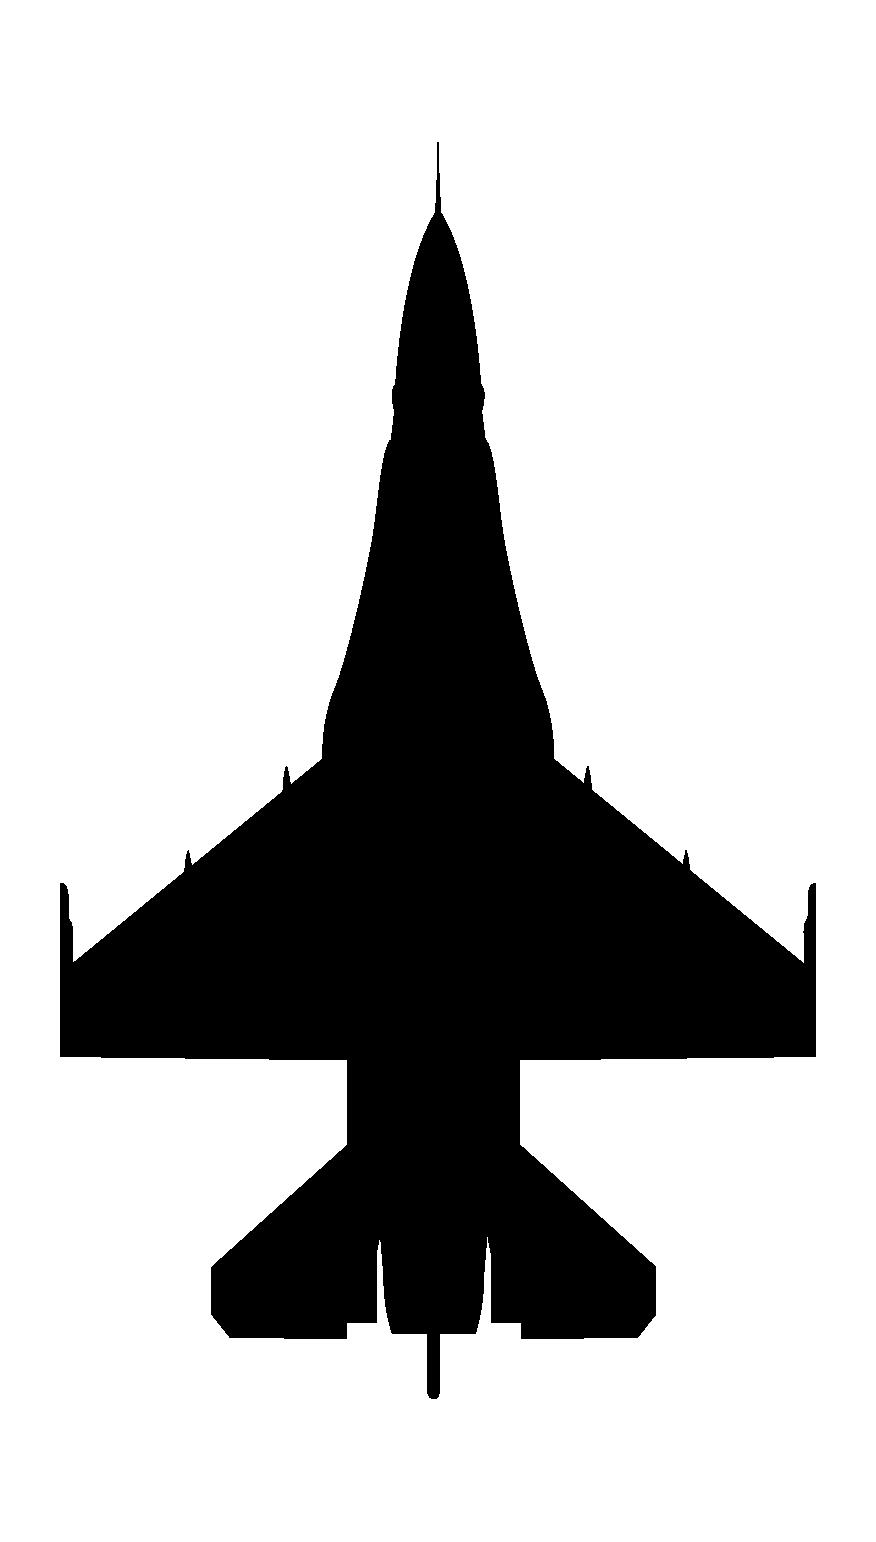
\includegraphics[
                    width=7.5mm,
                ]{diagrams/aircraft/silhouette_f16_top.pdf}
            };

            \node[yshift=-2mm] (3fig) at (3) {
                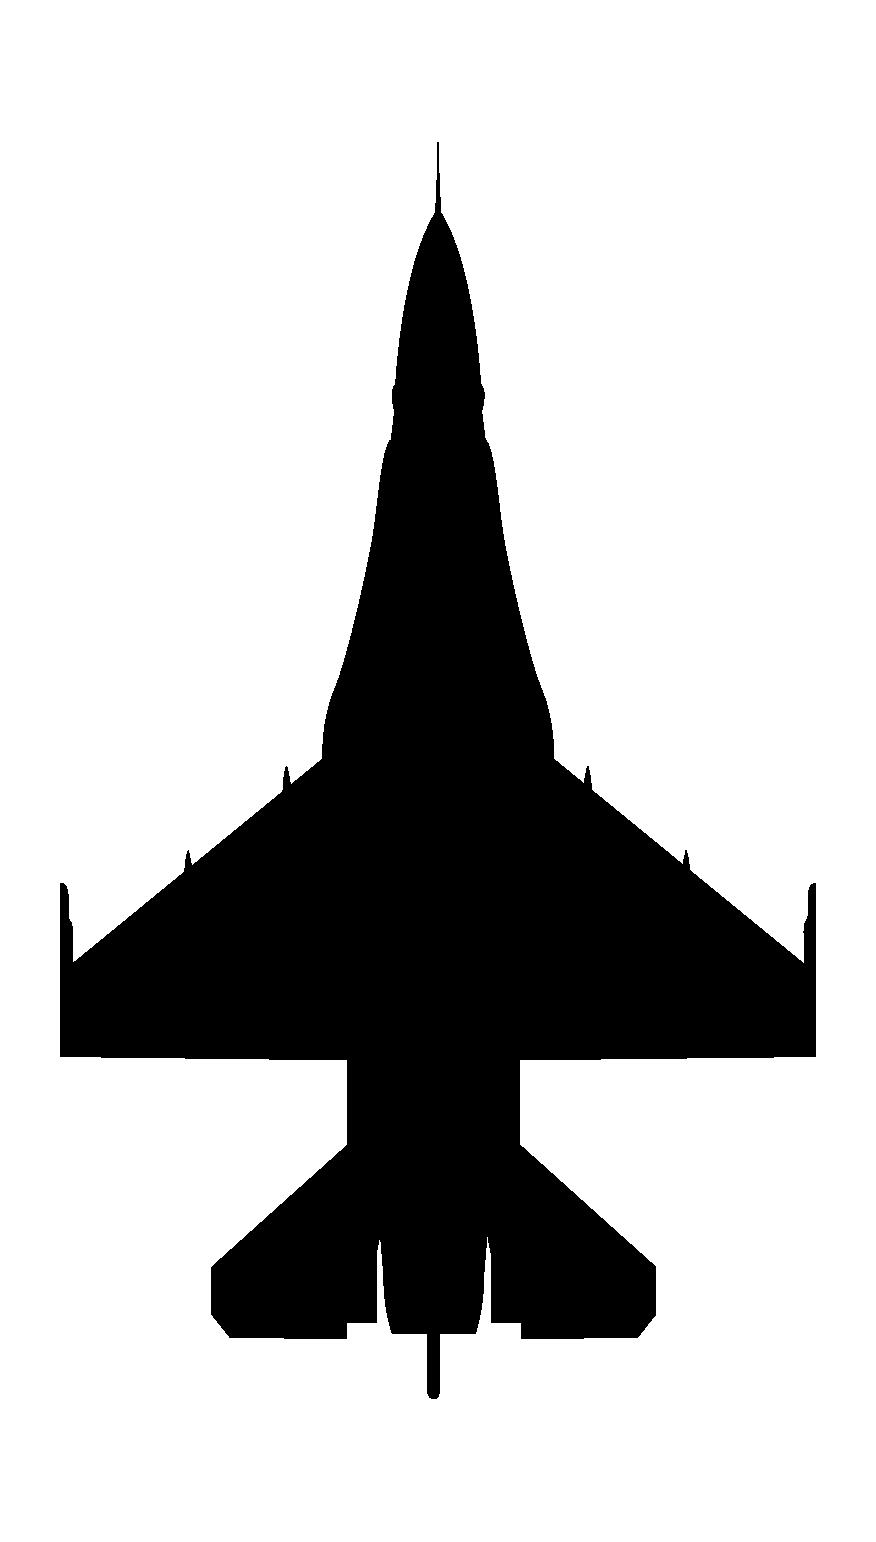
\includegraphics[
                    width=7.5mm,
                ]{diagrams/aircraft/silhouette_f16_top.pdf}
            };
            
            \node[yshift=-2mm] (4fig) at (4) {
                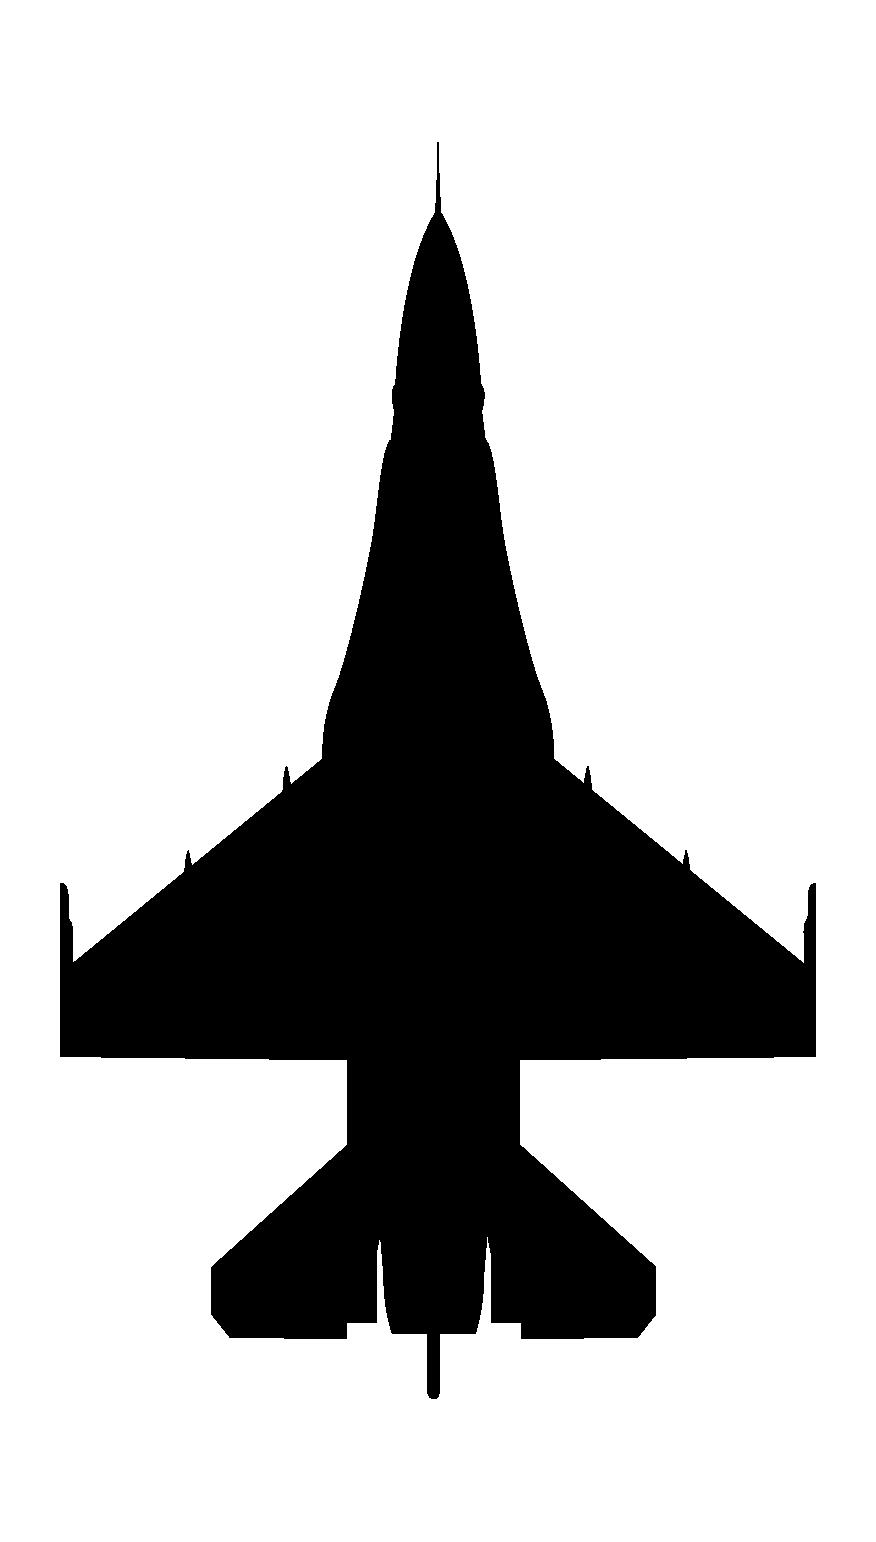
\includegraphics[
                    width=7.5mm,
                ]{diagrams/aircraft/silhouette_f16_top.pdf}
            };

            \node[anchor=north, font=\footnotesize] (1label) at (1fig.south) {1};
            \node[anchor=north, font=\footnotesize] (2label) at (2fig.south) {2};
            \node[anchor=north, font=\footnotesize] (3label) at (3fig.south) {3};
            \node[anchor=north, font=\footnotesize] (4label) at (4fig.south) {4};

        \end{tikzpicture}
        \caption{Spread formation}
        \label{fig:supp_fig:form:spread}
    \end{minipage}
\end{figure}

\clearpage